% ============================================================
%  The Particle Model — Lesson Booklet (one section per lesson: A Reading · B Theory · C Practice · D Above level)
%  Year 7 (Year 8 extension)  |  Victorian Curriculum F–10 Version 2.0
%  Compile with: xelatex three times, then python3 fill.py Particle_Model_Lesson_Booklet_Yr7
% ============================================================
\documentclass[11pt,a5paper,twoside]{article}
\newcommand{\unitname}{Advanced Separation}\newcommand{\unitcaps}{ADVANCED SEPARATION}

% ── Fonts (compile with LuaLaTeX) ────────────────────────────────────────────
\usepackage{fontspec}
% Bundled fonts (in ./fonts/) so the document compiles anywhere with XeLaTeX/LuaLaTeX
\setmainfont{Lato}[                   % body — humanist sans (stands in for deck's Inter)
  Path=../fonts/, Extension=.ttf, Ligatures=TeX,
  UprightFont=Lato-Regular, ItalicFont=Lato-Italic,
  BoldFont=Lato-Bold, BoldItalicFont=Lato-BoldItalic ]
\newfontfamily\headingfont{Poppins}[  % display/headings — matches the slide decks
  Path=../fonts/, Extension=.ttf, Ligatures=TeX,
  UprightFont=Poppins-Regular, ItalicFont=Poppins-Italic,
  BoldFont=Poppins-Bold, BoldItalicFont=Poppins-BoldItalic ]
\setlength{\headheight}{22pt}

\usepackage[protrusion=true,expansion=false]{microtype}
\usepackage[a5paper, inner=17mm, outer=13mm, top=19mm, bottom=17mm, headheight=14pt, headsep=4mm, footskip=8mm]{geometry}
\usepackage{xcolor}
\usepackage{tikz}
\usetikzlibrary{arrows.meta, shapes.geometric, calc, positioning, decorations.pathreplacing}
\usepackage{tcolorbox}
\tcbuselibrary{skins, breakable, raster}
\usepackage{fancyhdr}
\usepackage{titlesec}
\usepackage{enumitem}
\usepackage{booktabs}
\usepackage{tabularx}
\usepackage{array}
\usepackage{colortbl}
\usepackage{multicol}
\usepackage{amsmath}
\usepackage{needspace}
% TikZ diagram macros are embedded below (just before \begin{document}) for easy editing.
\usepackage{longtable}
\usepackage{graphicx}
\usepackage{lastpage}
\usepackage{calc}
\usepackage{mdframed}
\usepackage{setspace}
\usepackage{ragged2e}
% PDF bookmarks: one per lesson (made in \sectiondiv) plus the cover and
% contents, and links from the contents table to each lesson.
% implicit=false: hyperref adds no anchors of its own (an anchor on each
% list item nudged lists down 1.5 mm, which would undo the page fill).
% hidelinks keeps the links invisible, so the printed pages are unchanged.
\usepackage[implicit=false, hidelinks,
  pdftitle={Advanced Separation},
  pdfsubject={Years 7–8 Science, Victorian Curriculum F–10 v2.0}]{hyperref}
\usepackage{bookmark} % writes the outline itself, which implicit=false switches off in hyperref
% hyperref 7.01 with implicit=false leaves \Hy@PageAnchorSlide undefined, which
% throws at \end{document} and stops fill.py (it builds with -halt-on-error).
\makeatletter\providecommand\Hy@PageAnchorSlide{}\makeatother

% ── Colour Palette ───────────────────────────────────────────────────────────
% Remapped to the slide-deck palette (names kept so body + diagrams cascade)
\definecolor{NavyBlue}   {HTML}{16305C}
\definecolor{MidBlue}    {HTML}{2E6FE0}
\definecolor{LightBlue}  {HTML}{E8F1FF}
\definecolor{TealGreen}  {HTML}{0F6E63}
\definecolor{LightGreen} {HTML}{E0F7F3}
\definecolor{GoldDark}   {HTML}{C77F12}
\definecolor{GoldLight}  {HTML}{FFF3DC}
\definecolor{PurpleDark} {HTML}{5B3FC0}
\definecolor{PurpleLight}{HTML}{EFE9FF}
\definecolor{OrangeDark} {HTML}{C9483D}
\definecolor{OrangeLight}{HTML}{FFE9E6}
\definecolor{MidGrey}    {HTML}{AEBED4}
\definecolor{LightGrey}  {HTML}{F2F5FA}
\definecolor{DarkGrey}   {HTML}{3A4759}
\definecolor{TableHead}  {HTML}{16305C}
\definecolor{RowAlt}     {HTML}{EEF4FF}
% Bright accent tints (deck) for bars, rules and chips
\definecolor{Blue}   {HTML}{2E6FE0}
\definecolor{Teal}   {HTML}{18A999}
\definecolor{Amber}  {HTML}{F5A623}
\definecolor{Coral}  {HTML}{FF6B5E}
\definecolor{Violet} {HTML}{7C5CE0}
\definecolor{Sky}    {HTML}{4DA3FF}
\definecolor{Ink}    {HTML}{16223A}
\definecolor{Line}   {HTML}{DDE5F0}
\definecolor{Paper}  {HTML}{FBFCFE}

% ── Page Style ───────────────────────────────────────────────────────────────
\pagestyle{fancy}
\fancyhf{}
\renewcommand{\headrulewidth}{0.4pt}
\renewcommand{\headrule}{\hbox to\headwidth{\color{NavyBlue}\leaders\hrule height \headrulewidth\hfill}}
\fancyhead[L]{\headingfont\small\color{NavyBlue}The Particle Model}
\fancyhead[R]{\headingfont\small\color{DarkGrey}Year 7 \textbar{} Victorian Curriculum F--10 v2.0}
\fancyfoot[C]{\headingfont\small\color{DarkGrey}\thepage\ \textbar{} \pageref{LastPage}}
\fancypagestyle{plain}{%
  \fancyhf{}
  \fancyfoot[C]{\headingfont\small\color{DarkGrey}\thepage\ \textbar{} \pageref{LastPage}}
  \renewcommand{\headrulewidth}{0pt}
}

% ── Section Formatting ───────────────────────────────────────────────────────
\titleformat{\section}
  {\headingfont\color{NavyBlue}\Large\bfseries}
  {}{0em}{}
  [{\color{Teal}\rule[0.6ex]{2.2em}{3pt}}{\color{Line}\rule[0.6ex]{\dimexpr\linewidth-2.2em\relax}{1pt}}]
\titlespacing{\section}{0pt}{18pt}{8pt}

\titleformat{\subsection}
  {\headingfont\color{MidBlue}\large\bfseries}
  {\thesubsection}{0.6em}{}
\titlespacing{\subsection}{0pt}{12pt}{4pt}

\titleformat{\subsubsection}
  {\headingfont\color{NavyBlue}\normalsize\bfseries}
  {}{0em}{}
\titlespacing{\subsubsection}{0pt}{8pt}{2pt}

% Deck-style eyebrow / kicker (optional use)
\newcommand{\kicker}[2][Teal]{%
  {\headingfont\bfseries\footnotesize\color{#1}%
   \textcolor{#1}{\rule[0.18ex]{1.6em}{2.2pt}}\hspace{0.5em}\MakeUppercase{#2}\par}%
  \vspace{2pt}}

% ── Custom tcolorbox Environments ────────────────────────────────────────────

% Section divider banner
\newtcolorbox{sectionbanner}[2]{
  enhanced, breakable=false,
  colback=NavyBlue, colframe=NavyBlue,
  fontupper=\color{white}\bfseries\large,
  left=4mm, right=4mm, top=3mm, bottom=3mm,
  title={\color{white}\Huge\bfseries #1},
  attach boxed title to top left={yshift=-2mm, xshift=4mm},
  boxed title style={colback=NavyBlue, colframe=NavyBlue},
  after upper={\par\smallskip\normalfont\normalsize\color{white!80!NavyBlue}\textit{#2}}
}

% Key info box (blue)
\newtcolorbox{infobox}[1]{
  breakable, arc=2.5mm, boxrule=0.5pt,
  colback=LightBlue, colframe=Blue!40,
  fonttitle=\headingfont\bfseries, coltitle=MidBlue,
  title={#1},
  left=4mm, right=3.5mm, top=2.5mm, bottom=2.5mm
}

% Scaffold box (yellow)
\newtcolorbox{scaffold}[1]{
  breakable, arc=2.5mm, boxrule=0.5pt,
  colback=GoldLight, colframe=Amber!40,
  fonttitle=\headingfont\bfseries, coltitle=GoldDark,
  title={#1},
  left=4mm, right=3.5mm, top=2.5mm, bottom=2.5mm
}

% Worked example box
\newtcolorbox{workedexbox}[1]{
  breakable, arc=2.5mm, boxrule=0.5pt,
  colback=white, colframe=Amber!50,
  fonttitle=\headingfont\bfseries, coltitle=GoldDark,
  title={#1},
  left=4mm, right=3.5mm, top=2.5mm, bottom=2.5mm
}
% Worked examples: \begin{workedex}{title} -> "Worked Example N.M --- title",
% auto-numbered per section and labelled we:N.M. Never type the number.
\newcounter{wenum}[section]
\renewcommand{\thewenum}{\thesection.\arabic{wenum}}
\newenvironment{workedex}[1]
  {\refstepcounter{wenum}\label{we:\thewenum}\begin{workedexbox}{Worked Example \thewenum\ --- #1}}
  {\end{workedexbox}}

% We do: straight after each worked example, a near-identical question the
% class works through together, with its own writing space. Numbered to
% match the worked example above it and labelled wd:N.M.
%   \begin{wedo}{title} question ... \answerbox{h} \end{wedo}
\newtcolorbox{wedobox}[1]{
  enhanced, breakable=false, arc=2.5mm, boxrule=0.5pt,
  colback=white, colframe=TealGreen!55,
  fonttitle=\headingfont\bfseries, coltitle=TealGreen!75!black,
  title={#1},
  left=4mm, right=3.5mm, top=2.5mm, bottom=2.5mm
}
\newenvironment{wedo}[1]
  {\par\needspace{9\baselineskip}\begin{wedobox}{We do \thewenum\ --- #1}\label{wd:\thewenum}\ignorespaces}
  {\end{wedobox}}

% Year 7 box (blue)
\newtcolorbox{yr7box}{
  breakable, arc=2.5mm, boxrule=0.5pt,
  colback=LightBlue, colframe=Blue!40,
  left=4mm, right=3.5mm, top=2.5mm, bottom=2.5mm
}

% Year 8 extension box (violet)
\newtcolorbox{yr8box}{
  breakable, arc=2.5mm, boxrule=0.5pt,
  colback=PurpleLight, colframe=Violet!40,
  left=4mm, right=3.5mm, top=2.5mm, bottom=2.5mm
}

% Answer lines box
\newcommand{\answerbox}[1]{%
  \begin{tcolorbox}[
    enhanced, breakable, arc=2mm,
    colback=Paper, colframe=Line,
    left=2mm, right=2mm, top=1mm, bottom=1mm,
    boxrule=1pt,
    height=#1
  ]
  \end{tcolorbox}%
}

% Experiment header
\newtcolorbox{expheader}[3]{
  breakable=false, arc=2.5mm,
  colback=RowAlt, colframe=Amber!50, boxrule=0.5pt,
  fonttitle=\headingfont\bfseries\large, coltitle=NavyBlue,
  title={Experiment #1: #2},
  left=4mm, right=3.5mm, top=2.5mm, bottom=2.5mm,
  after upper={\par\smallskip
    {\headingfont\bfseries\color{GoldDark}Aim:}\ \textit{#3}},
}

% Reading comprehension passage box (green)
\newtcolorbox{readingbox}[1]{
  breakable, arc=2.5mm, boxrule=0.5pt,
  colback=white, colframe=Teal!50,
  fonttitle=\headingfont\bfseries, coltitle=TealGreen,
  title={#1},
  left=4mm, right=3.5mm, top=2.5mm, bottom=2.5mm,
  fontupper=\normalsize
}

% Skill-builder box (for beginner scaffolding)
\newtcolorbox{skillbox}[1]{
  breakable, arc=2.5mm, boxrule=0.5pt,
  colback=RowAlt, colframe=Blue!40,
  fonttitle=\headingfont\bfseries, coltitle=MidBlue,
  title={#1},
  left=4mm, right=3.5mm, top=2.5mm, bottom=2.5mm
}

% ── Custom Commands ───────────────────────────────────────────────────────────

% Question: \question{marks}{text}  (marks can be empty)
% Numbered automatically as Q<section>.<n>, reset every section.
% Do NOT write numbers by hand.
\newcounter{qnum}[section]
\renewcommand{\theqnum}{\thesection.\arabic{qnum}}
\newcommand{\question}[2]{%
  \refstepcounter{qnum}%
  \needspace{3\baselineskip}%
  \medskip
  \noindent\label{q:\theqnum}\textbf{Q\theqnum}\ifx&#1&\else\ \textcolor{DarkGrey}{(#1 mark\ifnum#1=1\else s\fi)}\fi\quad #2%
  \medskip
}

% Inline marks note
\newcommand{\markscount}[1]{\hfill\textcolor{DarkGrey}{\textit{(#1 mark\ifnum#1=1\else s\fi)}}}

% ── Practice set counter and question macros ─────────────────────────────────
\newcounter{pqnum}
\newcommand{\practiceset}[1]{%
  \needspace{6\baselineskip}
  \setcounter{pqnum}{0}%
  \vspace{6pt}
  {\headingfont\bfseries\large\color{GoldDark} Practice Set --- #1}\\[-2pt]
  {\color{Amber}\rule{\linewidth}{1pt}}\\[2pt]
}
% \pq{question text}{working box height}
\newcommand{\pq}[2]{%
  \stepcounter{pqnum}%
  \needspace{4\baselineskip}
  \vspace{5pt}
  \noindent\textbf{\thepqnum.}\quad #1\par
  \vspace{2pt}
  \answerbox{#2}
}
% Two short questions side by side, each with its own box
\newcommand{\pqpair}[4]{%
  \needspace{4\baselineskip}
  \vspace{5pt}
  \noindent
  \begin{minipage}[t]{0.48\linewidth}
    \stepcounter{pqnum}\textbf{\thepqnum.}\quad #1\par\vspace{2pt}
    \begin{tcolorbox}[enhanced,arc=2mm,colback=Paper,colframe=Line,left=2mm,right=2mm,
      top=1mm,bottom=1mm,boxrule=1pt,height=#2]\end{tcolorbox}
  \end{minipage}\hfill
  \begin{minipage}[t]{0.48\linewidth}
    \stepcounter{pqnum}\textbf{\thepqnum.}\quad #3\par\vspace{2pt}
    \begin{tcolorbox}[enhanced,arc=2mm,colback=Paper,colframe=Line,left=2mm,right=2mm,
      top=1mm,bottom=1mm,boxrule=1pt,height=#4]\end{tcolorbox}
  \end{minipage}
}

% ── Comprehension question macro (compact, lined) ────────────────────────────
\newcounter{rcnum}
\newcommand{\rcreset}{\setcounter{rcnum}{0}}
\newcommand{\rcq}[2]{%
  \stepcounter{rcnum}%
  \needspace{3\baselineskip}
  \vspace{4pt}
  \noindent\textbf{C\thercnum.}\quad #1\par
  \vspace{2pt}
  \linedbox{#2}
}

% Section divider (big numbered banner): \sectiondiv{title}{summary}
%
% This IS the section: it steps the real section counter, so subsections,
% tasks, questions and figures inside it are numbered N.M automatically.
% Put \label{sec:N} straight after it. Never hand-type a section number.
\newcommand{\sectiondiv}[2]{%
  \needspace{5\baselineskip}%
  \refstepcounter{section}%
  % PDF bookmark for the lesson; its anchor, lesson.N.1, is what the contents table links to
  \pdfbookmark[1]{Lesson \thesection{} — #1}{lesson.\thesection}%
  \begin{tcolorbox}[
    enhanced, breakable=false, arc=3.5mm,
    colback=NavyBlue, colframe=NavyBlue, boxrule=0pt,
    sidebyside, sidebyside align=center,
    lefthand width=2.4cm,
    left=2mm, right=4mm, top=4mm, bottom=4mm
  ]
    \begin{center}
      {\headingfont\bfseries\color{white!35!NavyBlue}\fontsize{50}{50}\selectfont \thesection}
    \end{center}
    \tcblower
    {\headingfont\bfseries\color{white}\LARGE #1}\\[3pt]
    {\itshape\color{white!75!NavyBlue}\small #2}
  \end{tcolorbox}%
}

% Tasks: \task, \task[a] (part a of a NEW task), \taskpart{b} (next part
% of the same task), \exttask (Year 8 "Extension" — same counter).
% Numbered Task <section>.<n>, reset every section. Do NOT type numbers.
% Every task, question and figure also gets an automatic label
% (task:1.7b, q:2.4, fig:1.2, fig:E2.1) so page refs come from the .aux.
\newcounter{tasknum}[section]
\renewcommand{\thetasknum}{\thesection.\arabic{tasknum}}
\NewDocumentCommand{\task}{o}{\refstepcounter{tasknum}\label{task:\thetasknum\IfValueT{#1}{#1}}\textbf{Task \thetasknum\IfValueT{#1}{#1}}}
\newcommand{\taskpart}[1]{\label{task:\thetasknum#1}\textbf{Task \thetasknum#1}}
\newcommand{\exttask}{\refstepcounter{tasknum}\label{task:\thetasknum}\textbf{Extension \thetasknum}}

% Figure captions: \figcap[fig:label]{caption} -> "Figure N.M --- caption"
% \expfigcap{caption} -> "Figure EN.M" (experiment pages). Both auto-numbered.
\newcounter{fignum}[section]
\renewcommand{\thefignum}{\thesection.\arabic{fignum}}
\newcounter{expfignum}[section]
\renewcommand{\theexpfignum}{E\thesection.\arabic{expfignum}}
\newcommand{\figcap}[2][]{%
  \begin{center}
    \refstepcounter{fignum}\label{fig:\thefignum}\if\relax\detokenize{#1}\relax\else\label{#1}\fi
    \small\itshape\color{DarkGrey} Figure \thefignum\ --- #2
  \end{center}%
}
\newcommand{\expfigcap}[1]{%
  \begin{center}
    \refstepcounter{expfignum}\label{fig:\theexpfignum}%
    \small\itshape\color{DarkGrey} Figure \theexpfignum\ --- #1
  \end{center}%
}

% Diagram include
\newcommand{\diagramfig}[3]{%  {filename}{width fraction}{caption}
  \begin{center}
    \includegraphics[width=#2\linewidth]{#1}\\[4pt]
    \small\itshape\color{DarkGrey} #3
  \end{center}%
}

% Table column types
\newcolumntype{L}[1]{>{\RaggedRight\arraybackslash}p{#1}}
\newcolumntype{C}[1]{>{\Centering\arraybackslash}p{#1}}

% Table header colour
\newcommand{\thead}[1]{\cellcolor{TableHead}\color{white}\bfseries #1}
\newcommand{\talt}{\rowcolor{RowAlt}}
\newcommand{\tmid}{\rowcolor{MidGrey}}

% Inline year tags
\newcommand{\tagyr}[1]{%
  \tikz[baseline=-0.5ex]\node[
    rounded corners=2pt,
    fill=#1!20, draw=#1, text=#1,
    inner xsep=4pt, inner ysep=1pt,
    font=\scriptsize\bfseries
  ]{Yr #1 only};}

% Draw answer lines
\newcommand{\anslines}[1]{%
  \vspace{2pt}%
  \foreach \n in {1,...,#1}{%
    \par\noindent\rule{\linewidth}{0.3pt}\vspace{3pt}%
  }%
}

% ── Document ─────────────────────────────────────────────────────────────────
% ── Optional-lesson note, shown under the lesson banner ──────────────────────
\newcommand{\optionalnote}[1]{%
  % the title is a bold lead-in on the first line rather than a title bar,
  % which keeps Lesson 11's reading on the lesson's first page
  \begin{tcolorbox}[enhanced, breakable=false, arc=2.5mm, boxrule=0.5pt,
    colback=PurpleLight, colframe=Violet!50,
    left=4mm, right=3.5mm, top=2mm, bottom=2mm]
  {\headingfont\bfseries\color{PurpleDark}Optional lesson \textbullet{} Year 8 extension.}\enspace #1
  \end{tcolorbox}\vspace{2pt}}


% ══════════════════════════════════════════════════════════════════════════════
%  LESSON STRUCTURE (lesson booklet, Oct 2026)
%  Every lesson runs in the same four parts, in this order:
%    \lessonpart{A}{Reading and comprehension}{Teal}   \label{read:N}
%    \lessonpart{B}{Theory and examples}{Blue}         \label{theory:N}
%    \lessonpart{C}{Practice}{Amber}                    \label{prac:N}
%    \lessonpart{D}{Above level}{Violet}                \label{ext:N}
%  Above-level / higher-order questions live ONLY in Part D, at the end.
% ══════════════════════════════════════════════════════════════════════════════
\newcommand{\lessonpart}[3]{%
  \par\if#1A\needspace{10\baselineskip}\vspace{10pt}\else
    \if#1C\notesfill\fi\clearpage\fi
  \begin{tcolorbox}[enhanced, breakable=false, arc=2mm, boxrule=0pt,
    colback=#3!14, borderline west={4pt}{0pt}{#3},
    left=4mm, right=3mm, top=1.6mm, bottom=1.6mm]
  {\headingfont\bfseries\color{#3!60!black}\large Part #1 \textbullet{} #2}
  \end{tcolorbox}\vspace{2pt}}

% Key vocabulary at the start of each lesson: students copy each definition
% from the vocabulary slide in the lesson's starter. First row = red scaffold.
\newcommand{\vocabhead}{%
  \par\vspace{6pt}%
  \begin{tcolorbox}[enhanced, breakable=false, arc=2mm, boxrule=0pt,
    colback=NavyBlue!10, borderline west={4pt}{0pt}{NavyBlue},
    left=4mm, right=3mm, top=1.6mm, bottom=1.6mm]
  {\headingfont\bfseries\color{NavyBlue}\large Key vocabulary}
  \end{tcolorbox}\vspace{2pt}%
  \noindent Copy the definition of each word from the slide. The first one has been done for you.\par}

% Curriculum codes under a lesson banner
\newcommand{\lessoncodes}[1]{%
  {\small\headingfont\color{DarkGrey}Victorian Curriculum 2.0:\ \textbf{#1}}\par\vspace{4pt}}

% Two short tasks side by side, each with its own working box
% \taskpair{text}{box height}{text}{box height}
% The two boxes line up: the shorter question is padded by the difference in
% text height (measured in a scratch box, task counter restored, no label).
\newsavebox\tpbox
\newlength\tpA \newlength\tpB
\newcount\tpsaved
\newcommand\tpmeasure[2]{%
  \tpsaved=\value{tasknum}%
  \sbox\tpbox{\vbox{\hsize=0.485\linewidth \linewidth=\hsize \parskip=0pt
    \renewcommand\label[1]{}\task #1\par}}%
  \setlength{#2}{\dimexpr\ht\tpbox+\dp\tpbox\relax}%
  \setcounter{tasknum}{\tpsaved}}
\newcommand{\taskpair}[4]{%
  \par\needspace{9\baselineskip}\vspace{4pt}%
  \tpmeasure{#1}{\tpA}\tpmeasure{#3}{\tpB}%
  \noindent
  \edef\abgrp{\number\numexpr\value{abox}+1\relax}%
  \begin{minipage}[t]{0.485\linewidth}
    \task #1\par\ifdim\tpB>\tpA\vspace{\dimexpr\tpB-\tpA\relax}\fi\vspace{2pt}\answerbox{#2}
  \end{minipage}\hfill
  \begin{minipage}[t]{0.485\linewidth}
    \task #3\par\ifdim\tpA>\tpB\vspace{\dimexpr\tpA-\tpB\relax}\fi\vspace{2pt}\answerbox{#4}
  \end{minipage}\par\gdef\abgrp{0}\vspace{4pt}}
% Two parts of one question side by side, with their answer boxes level:
% \ptpair{a}{part (a) text}{box height}{b}{part (b) text}{box height}.
% The shorter part's text gets space below it to match the longer one.
\newcommand\ptmeasure[3]{%
  \sbox\tpbox{\vbox{\hsize=0.485\linewidth \linewidth=\hsize \parskip=0pt \pt{#1}#2\par}}%
  \setlength{#3}{\dimexpr\ht\tpbox+\dp\tpbox\relax}}
\newcommand{\ptpair}[6]{%
  \ptmeasure{#1}{#2}{\tpA}\ptmeasure{#4}{#5}{\tpB}%
  \par\noindent
  \edef\abgrp{\number\numexpr\value{abox}+1\relax}%
  \begin{minipage}[t]{0.485\linewidth}
    \pt{#1}#2\par\ifdim\tpB>\tpA\vspace{\dimexpr\tpB-\tpA\relax}\fi\answerbox{#3}
  \end{minipage}\hfill
  \begin{minipage}[t]{0.485\linewidth}
    \pt{#4}#5\par\ifdim\tpA>\tpB\vspace{\dimexpr\tpA-\tpB\relax}\fi\answerbox{#6}
  \end{minipage}\par\gdef\abgrp{0}}

% Answer boxes never split across a page (a half box on its own page is useless)
% ── Page filling ────────────────────────────────────────────────────────────
% Every writing box gets an id. Its page is logged to \jobname.abp; fill.py
% measures the empty space left at the foot of each page and shares it out
% among that page's boxes via \jobname.abx (\abset{id}{extra}). Side-by-side
% boxes share a group so they grow together.
\newcounter{abox}
\newwrite\abpos \immediate\openout\abpos=\jobname.abp
\newcommand{\abset}[2]{\expandafter\gdef\csname abx@#1\endcsname{#2}}
\InputIfFileExists{\jobname.abx}{}{}
\def\abgrp{0}
\newcommand{\abnext}{\stepcounter{abox}%
  \edef\abcur{\ifcsname abx@\theabox\endcsname\csname abx@\theabox\endcsname\else 0pt\fi}}
\newcommand{\ablog}{\edef\abtmp{\noexpand\write\abpos{\theabox\space\abgrp\space\noexpand\thepage}}\abtmp}
\newcommand{\abh}[1]{\dimexpr#1+\abcur\relax}
\renewcommand{\answerbox}[1]{%
  \abnext
  \begin{tcolorbox}[enhanced, breakable=false, arc=2mm, colback=Paper, colframe=Line,
    left=2mm, right=2mm, top=1mm, bottom=1mm, boxrule=1pt, height=\abh{#1}]
  \end{tcolorbox}\ablog%
}
% \linedbox{height}: an answer box ruled in dotted thirds. Lines are \thirdrow/3 apart and run dotted, dotted,
% solid (the baseline), repeating, and end on one dotted line. The number of
% rows is worked out from the box's final height, so the ruling still fills the
% box after fill.py has grown it; the rows are centred in the box.
\newlength\thirdrow \setlength\thirdrow{9mm}
\tikzset{thirdsolid/.style={draw=DarkGrey!70, line width=0.5pt},
         thirddot/.style={draw=DarkGrey!70, line width=0.6pt, dash pattern=on 0.9pt off 1.6pt}}
\newlength\lbH \newlength\lbO \newcount\lbN
\newcommand{\linedbox}[1]{%
  \abnext
  % interior height = box height less the 1pt frame top and bottom
  \setlength\lbH{\dimexpr\abh{#1}-2pt\relax}%
  % whole rows that fit with at least 3 mm spare top and bottom (at least one)
  \lbN=\numexpr(\dimexpr\lbH-6mm-\thirdrow/2\relax)/\thirdrow\relax
  \ifnum\lbN<1 \lbN=1 \fi
  \setlength\lbO{\dimexpr(\lbH-\lbN\thirdrow)/2\relax}%
  \begin{tcolorbox}[enhanced, breakable=false, arc=2mm, colback=Paper, colframe=Line,
    left=2mm, right=2mm, top=1mm, bottom=1mm, boxrule=1pt, height=\abh{#1},
    underlay={\begin{tcbclipinterior}
      \foreach \i in {1,...,\the\lbN}{
        \draw[thirddot] ([xshift=3mm,yshift=-\lbO-(\i-1)*\thirdrow]interior.north west) -- ([xshift=-3mm,yshift=-\lbO-(\i-1)*\thirdrow]interior.north east);
        \draw[thirddot] ([xshift=3mm,yshift=-\lbO-(\i-1)*\thirdrow-\thirdrow/3]interior.north west) -- ([xshift=-3mm,yshift=-\lbO-(\i-1)*\thirdrow-\thirdrow/3]interior.north east);
        \draw[thirdsolid] ([xshift=3mm,yshift=-\lbO-(\i-1)*\thirdrow-2*\thirdrow/3]interior.north west) -- ([xshift=-3mm,yshift=-\lbO-(\i-1)*\thirdrow-2*\thirdrow/3]interior.north east);}
      \draw[thirddot] ([xshift=3mm,yshift=-\lbO-\lbN\thirdrow]interior.north west) -- ([xshift=-3mm,yshift=-\lbO-\lbN\thirdrow]interior.north east);
    \end{tcbclipinterior}}]
  \end{tcolorbox}\ablog%
}
% Every written-response box is ruled the same way (Part A comprehension, We do,
% Part C tasks and Part D extensions, including side-by-side pairs). Space for
% mathematical working uses \workbox{height} instead and stays plain, as do
% \drawbox and the write-in tables.
\let\workbox\answerbox   % plain box: mathematical working (calculations) stays unruled
\let\answerbox\linedbox
% \drawbox{height}{contents}: white box for a diagram or drawing
\newcommand{\drawbox}[2]{%
  \abnext
  \begin{tcolorbox}[colback=white, colframe=MidGrey, boxrule=0.5pt, height=\abh{#1}]#2\end{tcolorbox}\ablog}
% Notes box at the end of Part B: fills whatever is left of the page (if worth it)
\newcommand{\notesfill}{\par
  \ifdim\dimexpr\pagegoal-\pagetotal\relax>3.2cm
    \vspace*{\fill}%
    \begin{tcolorbox}[enhanced, breakable=false, arc=2mm, colback=Paper, colframe=Line,
      left=2mm, right=2mm, top=1mm, bottom=1mm, boxrule=1pt,
      height=\dimexpr\pagegoal-\pagetotal-1.0cm\relax]
      {\small\headingfont\color{DarkGrey}Notes}
    \end{tcolorbox}%
  \fi}



% Centred table: wrap every content table in \begin{ctab} ... \end{ctab}
% (figures already centre themselves inside their \diag... macros)
% ctab also registers write-in tables (S column) for page filling: the extra
% height is per row, logged with the row count.
\newenvironment{ctab}{\par\smallskip\begingroup\centering
  \abnext\let\tbcur\abcur\global\wtrows0 }{\par
  \ifnum\wtrows>0 \edef\abtmp{\noexpand\write\abpos{\theabox\space\abgrp\space\noexpand\thepage\space\the\wtrows}}\abtmp\fi
  \endgroup\smallskip}

% ── Booklet formatting rules (Oct 2026) ─────────────────────────────────────
% 1. No marks are shown anywhere in the booklet.
\renewcommand{\markscount}[1]{}
% 2. A task's heading sits on its own line; its text starts on the next
%    line, left aligned. Parts (a), (b)… each start a new line: use \pt{a}.
\RenewDocumentCommand{\task}{o}{\par\noindent\refstepcounter{tasknum}\label{task:\thetasknum\IfValueT{#1}{#1}}\textbf{Task \thetasknum\IfValueT{#1}{#1}}\par\nobreak\noindent\ignorespaces}
\renewcommand{\taskpart}[1]{\par\noindent\label{task:\thetasknum#1}\textbf{Task \thetasknum#1}\par\nobreak\noindent\ignorespaces}
\renewcommand{\exttask}{\par\noindent\refstepcounter{tasknum}\label{task:\thetasknum}\textbf{Extension \thetasknum}\par\nobreak\noindent\ignorespaces}
\newcommand{\pt}[1]{\par\noindent\textbf{(#1)}\ \ignorespaces}
% Workstation pages (Experiment 1): numbered method steps with a hanging
% indent, and a one-line safety reminder under the materials list.
\newcommand{\wsstep}[1]{\par\noindent\hangindent=1.6em\hangafter=1\makebox[1.6em][l]{\textbf{#1}}\ignorespaces}
\newcommand{\wssafety}[1]{\par\smallskip{\small\textcolor{ScaffoldRed}{\headingfont\bfseries Safety:}\ #1}\par}
% 3. Tables have vertical rules between columns and down both sides
%    (write | between and around the columns, e.g. {|L{3cm}|C{2cm}|}).
%    Keep the normal padding at the outer edges (no @{} there): colortbl paints
%    header colour one \tabcolsep past each edge, so trimming the padding makes
%    the header overhang the grid.
\arrayrulecolor{MidGrey}
\setlength{\arrayrulewidth}{0.6pt}
% 4. Write-in tables: W/Z are left/centred columns that centre text
%    vertically; put the S column first (see below).
\newcolumntype{W}[1]{>{\RaggedRight\arraybackslash}m{#1}}
\newcolumntype{Z}[1]{>{\Centering\arraybackslash}m{#1}}
\def\tbcur{0pt}
\newcount\wtrows
\newcommand{\wh}{\global\advance\wtrows1 \rule[\dimexpr-0.75cm-\tbcur/2\relax]{0pt}{\dimexpr1.5cm+\tbcur\relax}}
% S = zero-width first column that makes every row of a write-in table
% at least 1.5 cm tall with its text vertically centred. Start each data
% row with "&"; start the header row with "\hd &" so it stays slim.
\newif\ifnowh
\newcolumntype{S}{@{}>{}c<{\ifnowh\else\wh\fi\global\nowhfalse}@{\hspace{\tabcolsep}}}
\newcommand{\hd}{\global\nowhtrue}
% 5. The first row of a multi-row write-in table is a worked scaffold in red.
\definecolor{ScaffoldRed}{HTML}{C0392B}
\newcommand{\scaf}[1]{\textcolor{ScaffoldRed}{\itshape #1}}
% 6. Tables are a light grid (rules between rows and columns) on white —
%    row shading is off, because colortbl paints shading over column rules.
\renewcommand{\talt}{}
\renewcommand{\tmid}{}
% ══════════════════════════════════════════════════════════════════════════════
%  DIAGRAM DEFINITIONS — The Particle Model
%  Self-contained TikZ macros, no external image files. Each \diag... macro is
%  called from the body by name.
% ══════════════════════════════════════════════════════════════════════════════
\usetikzlibrary{arrows.meta,calc,positioning,patterns,backgrounds}
\tikzset{
  thin arrow/.style={-{Stealth[length=6pt,width=4pt]}, line width=1.4pt},
}

% ── Lesson 1: the same three jars holding a solid, a liquid and a gas ───────────
% The solid keeps its own shape, the liquid takes the jar's shape with a flat top,
% the gas fills the whole jar. No particles yet: those arrive in Lesson 4.
\newcommand{\jar}[1]{% jar outline with its base at (#1,0)
  \draw[line width=1.2pt, Ink] (#1-1.25,2.9) -- (#1-1.25,0.15) arc (180:270:0.15)
    -- (#1+1.1,0) arc (270:360:0.15) -- (#1+1.25,2.9);}
\newcommand{\diagStates}{%
\begin{center}
\begin{fitbox}\begin{tikzpicture}[font=\small, x=1cm, y=1cm]
  % solid: a block sitting in the corner
  \fill[GoldLight] (-0.95,0.02) rectangle (0.15,1.25);
  \draw[GoldDark, line width=1.1pt] (-0.95,0.02) rectangle (0.15,1.25);
  \jar{0}
  \node[font=\bfseries, text=NavyBlue] at (0,-0.45) {Solid};
  \node[align=center, font=\footnotesize, text=DarkGrey] at (0,-1.05) {keeps its own shape\\and volume};
  % liquid: takes the jar's shape, flat top
  \begin{scope}[xshift=4.2cm]
    \fill[Sky!35] (-1.25,0.15) arc (180:270:0.15) -- (1.1,0) arc (270:360:0.15) -- (1.25,1.1) -- (-1.25,1.1) -- cycle;
    \draw[MidBlue, line width=1.1pt] (-1.25,1.1) -- (1.25,1.1);
    \jar{0}
    \node[font=\bfseries, text=NavyBlue] at (0,-0.45) {Liquid};
    \node[align=center, font=\footnotesize, text=DarkGrey] at (0,-1.05) {takes the jar's shape,\\keeps its volume};
  \end{scope}
  % gas: fills the whole (sealed) jar
  \begin{scope}[xshift=8.4cm]
    \fill[Violet!16] (-1.25,0.15) arc (180:270:0.15) -- (1.1,0) arc (270:360:0.15) -- (1.25,2.9) -- (-1.25,2.9) -- cycle;
    \draw[line width=2.2pt, DarkGrey] (-1.4,2.9) -- (1.4,2.9);
    \jar{0}
    \node[font=\scriptsize, text=DarkGrey, anchor=south] at (0,2.95) {lid};
    \node[font=\bfseries, text=NavyBlue] at (0,-0.45) {Gas};
    \node[align=center, font=\footnotesize, text=DarkGrey] at (0,-1.05) {spreads out to fill\\the whole jar};
  \end{scope}
\end{tikzpicture}\end{fitbox}
\end{center}}

% ── Lesson 1, Worked Example 1.2 and We do 1.2: the same syringe, before and after
\newcommand{\diagSyringe}[3]{% {start mL}{end mL}{contents: gas|liquid}
\begin{center}\resizebox{\linewidth}{!}{%
\begin{fitbox}\begin{tikzpicture}[font=\scriptsize, x=0.11cm, y=1cm]
  \foreach \row/\vol/\lab in {0/#1/before, -1.15/#2/after}{
    \begin{scope}[yshift=\row cm]
      \ifx#3g\fill[Violet!16] (0,0) rectangle (\vol,0.7);\else\fill[Sky!35] (0,0) rectangle (\vol,0.7);\fi
      \draw[line width=1pt, Ink] (0,0) rectangle (60,0.7);
      \draw[line width=1pt, Ink] (0,0.25) -- (-4,0.25) (0,0.45) -- (-4,0.45);
      \fill[Ink] (-5.5,0.15) rectangle (-4,0.55);
      \foreach \t in {0,10,...,60}{\draw[Ink] (\t,0.7) -- (\t,0.85); \node[anchor=south, font=\tiny] at (\t,0.82) {\t};}
      \fill[DarkGrey] (\vol,0.04) rectangle (\vol+1.6,0.66);
      \draw[line width=2pt, DarkGrey] (\vol+1.6,0.35) -- (\vol+26,0.35);
      \draw[line width=2pt, DarkGrey] (\vol+26,0.05) -- (\vol+26,0.65);
      \node[anchor=east, font=\scriptsize\bfseries, text=DarkGrey] at (-7,0.35) {\lab};
    \end{scope}}
  \node[font=\tiny, text=DarkGrey, anchor=west] at (61,0.35) {mL};
  \node[font=\tiny, text=DarkGrey, anchor=north] at (-4.75,-1.2) {sealed tip};
\end{tikzpicture}\end{fitbox}}
\end{center}}

% needspace.sty reserves room by planting a penalty -100 with 9 lines of
% temporary stretch. On a page that can't be filled tightly that fake break
% always wins, so a We do that fitted was pushed over and left half a page
% empty. This version breaks only when the room really isn't there, and
% ragged bottom lets every other page run on until something won't fit;
% fill.py then grows the writing boxes into what is left at the foot.
\renewcommand{\needspace}[1]{\par\ifdim\dimexpr\pagegoal-\pagetotal\relax<\dimexpr#1\relax\newpage\fi}
\raggedbottom
% Part D sits in a breakable yr8box, where \needspace can't see the page (the box
% is built off the page first). Wrap each extension in keepext so it is one
% unsplittable block: the yr8box then breaks between extensions, never inside one.
\newenvironment{keepext}{\par\begin{tcolorbox}[blankest, breakable=false]}{\end{tcolorbox}\par}
% ══════════════════════════════════════════════════════════════════════════════
%  SHARED DIAGRAMS — particle boxes, graphs and lab apparatus (Lessons 2–27)
% ══════════════════════════════════════════════════════════════════════════════
% Particles are 3.2 mm discs. Solids and liquids hold about the same number of
% particles at the same spacing (touching): a liquid is NOT drawn more spread
% out than a solid, because that is the misconception Lesson 6 corrects.
\tikzset{
  pA/.style={circle, fill=Sky!55, draw=MidBlue, line width=0.5pt, minimum size=3.2mm, inner sep=0pt},
  pB/.style={circle, fill=Coral!50, draw=OrangeDark, line width=0.5pt, minimum size=3.2mm, inner sep=0pt},
  pC/.style={circle, fill=Amber!55, draw=GoldDark, line width=0.5pt, minimum size=3.2mm, inner sep=0pt},
  pD/.style={circle, fill=Teal!45, draw=TealGreen, line width=0.5pt, minimum size=3.2mm, inner sep=0pt},
  move/.style={-{Stealth[length=3pt,width=3pt]}, line width=0.7pt, DarkGrey},
  boxline/.style={line width=1pt, Ink},
  axis/.style={-{Stealth[length=5pt,width=4pt]}, line width=0.9pt, Ink},
  glass/.style={line width=1pt, Ink},
  lab/.style={font=\scriptsize, text=DarkGrey},
}
\makeatletter
% particle kinds, drawn at (#1,#2): A, B, C, D single particles; AA, BB, CC
% two joined; AB a joined pair; BAB a three-particle molecule.
\newcommand{\pk@A}[2]{\node[pA] at (#1,#2) {};}
\newcommand{\pk@B}[2]{\node[pB] at (#1,#2) {};}
\newcommand{\pk@C}[2]{\node[pC] at (#1,#2) {};}
\newcommand{\pk@D}[2]{\node[pD] at (#1,#2) {};}
\newcommand{\pk@AA}[2]{\node[pA] at ($(#1,#2)+(-0.13,0)$) {};\node[pA] at ($(#1,#2)+(0.13,0)$) {};}
\newcommand{\pk@BB}[2]{\node[pB] at ($(#1,#2)+(-0.13,0)$) {};\node[pB] at ($(#1,#2)+(0.13,0)$) {};}
\newcommand{\pk@CC}[2]{\node[pC] at ($(#1,#2)+(-0.13,0)$) {};\node[pC] at ($(#1,#2)+(0.13,0)$) {};}
\newcommand{\pk@AB}[2]{\node[pA] at ($(#1,#2)+(-0.13,0)$) {};\node[pB] at ($(#1,#2)+(0.13,0)$) {};}
\newcommand{\pk@BAB}[2]{\node[pB] at ($(#1,#2)+(-0.24,0)$) {};\node[pB] at ($(#1,#2)+(0.24,0)$) {};\node[pA] at (#1,#2) {};}
\newcommand{\pk}[3]{\csname pk@#1\endcsname{#2}{#3}}
\makeatother
% eight spread-out positions in a 2.6 cm box (for gases and particle diagrams)
\def\gaspos{0.55/0.55,1.55/0.45,2.15/1.05,0.75/1.35,1.65/1.5,0.5/2.1,2.1/2.15,1.3/2.05}
% the box: a 2.6 cm square with its bottom-left corner at the scope origin
\newcommand{\pbox}{\draw[boxline] (0,0) rectangle (2.6,2.6);}
% \pkinds{A,A,AB,...}: up to eight particles, placed at the eight gas positions
\newcommand{\pkinds}[1]{%
  \foreach \k [count=\i] in {#1}{%
    \foreach \x/\y [count=\j] in \gaspos{\ifnum\i=\j \pk{\k}{\x}{\y}\fi}}}
% \stateIn{solid|liquid|gas}{style} — the particles of one state, in a box
\newcommand{\stateIn}[2]{%
  \ifstrequal{#1}{solid}{%
    \foreach \r in {0,...,4}{\foreach \c in {0,...,6}{\node[#2] at (0.31+\c*0.33,0.2+\r*0.33) {};}}}{}%
  \ifstrequal{#1}{liquid}{%
    \foreach \x/\y in {2.29/0.20,0.42/0.20,1.28/0.20,0.85/0.20,1.87/0.20,1.07/0.47,1.45/0.49,0.28/0.51,0.72/0.52,2.34/0.54,1.87/0.54,1.29/0.80,2.03/0.85,0.27/0.86,0.69/0.86,1.68/0.90,2.34/0.98,0.88/1.15,2.01/1.20,1.63/1.24,0.55/1.26,1.18/1.31,2.36/1.33,0.23/1.39,0.88/1.50,1.99/1.55,1.65/1.59,0.51/1.61,1.30/1.63}{\node[#2] at (\x,\y) {};}}{}%
  \ifstrequal{#1}{gas}{%
    \foreach \x/\y in \gaspos{\node[#2] at (\x,\y) {};}}{}%
  \pbox}
% motion marks: short arrows for a gas, small wiggles for a solid
\newcommand{\gasMoves}{%
  \draw[move] (0.55,0.55)+(0.2,0.12) -- +(0.55,0.33);
  \draw[move] (1.55,0.45)+(-0.2,0.08) -- +(-0.55,0.25);
  \draw[move] (2.15,1.05)+(0,0.2) -- +(0.05,0.55);
  \draw[move] (0.75,1.35)+(0.2,-0.08) -- +(0.55,-0.2);
  \draw[move] (1.65,1.5)+(-0.18,0.12) -- +(-0.45,0.4);
  \draw[move] (0.5,2.1)+(0.08,-0.2) -- +(0.2,-0.52);
  \draw[move] (2.1,2.15)+(-0.2,-0.05) -- +(-0.55,-0.15);
  \draw[move] (1.3,2.05)+(0.12,0.15) -- +(0.3,0.38);}
\newcommand{\solidWiggles}{%
  \foreach \c in {1,3,5}{\draw[DarkGrey, line width=0.5pt] (0.31+\c*0.33-0.14,1.86) -- ++(0.07,0.06) -- ++(0.07,-0.06) -- ++(0.07,0.06) -- ++(0.07,-0.06);}}
\newcommand{\liquidMoves}{%
  \draw[move] (0.88,1.5)+(0.18,0.05) -- +(0.42,0.12);
  \draw[move] (1.99,1.55)+(-0.18,0.06) -- +(-0.42,0.14);
  \draw[move] (0.55,1.26)+(-0.05,0.18) -- +(-0.1,0.4);}

% Figure: the three states side by side, with movement marks
\newcommand{\diagThreeStates}{%
\begin{center}\begin{fitbox}\begin{tikzpicture}[font=\small]
  \begin{scope}\stateIn{solid}{pA}\solidWiggles\end{scope}
  \begin{scope}[xshift=4.2cm]\stateIn{liquid}{pA}\liquidMoves\end{scope}
  \begin{scope}[xshift=8.4cm]\stateIn{gas}{pA}\gasMoves\end{scope}
  \foreach \x/\t/\d in {1.3/Solid/{packed in a pattern,\\vibrate in place}, 5.5/Liquid/{close together, slide\\past each other}, 9.7/Gas/{far apart, move fast\\in every direction}}{
    \node[font=\bfseries, text=NavyBlue] at (\x,-0.35) {\t};
    \node[align=center, font=\footnotesize, text=DarkGrey] at (\x,-0.95) {\d};}
\end{tikzpicture}\end{fitbox}\end{center}}

% \pboxfig{tikz contents}{label}: one small labelled box (for tasks)
\newcommand{\pboxfig}[2]{%
  \begin{fitbox}\begin{tikzpicture}[baseline=(b.base)]#1\pbox
    \node[font=\small\bfseries, text=NavyBlue] (b) at (1.3,-0.35) {#2};\end{tikzpicture}\end{fitbox}}

% graph-paper box for drawing a graph: \graphgrid{height}
\newcommand{\graphgrid}[1]{%
  \begin{tcolorbox}[enhanced, breakable=false, colback=white, colframe=MidGrey, boxrule=0.5pt, height=#1,
    underlay={\begin{tcbclipinterior}\draw[step=5mm, Line, very thin] (interior.south west) grid (interior.north east);
      \draw[step=1cm, MidGrey!70, thin] (interior.south west) grid (interior.north east);\end{tcbclipinterior}}]
  \end{tcolorbox}}

% Heating curve for water, -20 °C ice to steam at 120 °C. #1 = labels on (1) / off (0)
\newcommand{\diagHeatingCurve}[1]{%
\begin{center}\begin{fitbox}\begin{tikzpicture}[x=0.95cm, y=0.032cm, font=\footnotesize]
  \foreach \t in {-20,0,20,...,120}{\draw[Line] (0,\t) -- (11,\t); \node[anchor=east, text=DarkGrey] at (0,\t) {\t};}
  \foreach \m in {0,...,11}{\draw[Line] (\m,-20) -- (\m,120);}
  \foreach \m in {0,2,...,10}{\node[anchor=north, text=DarkGrey] at (\m,-20) {\m};}
  \draw[axis] (0,-20) -- (11.4,-20) node[anchor=north east, yshift=-12pt, text=Ink] {time (minutes)};
  \draw[axis] (0,-20) -- (0,132) node[anchor=south, text=Ink] {temperature (\textdegree C)};
  \draw[line width=1.8pt, OrangeDark, line join=round] (0,-20) -- (1,0) -- (3,0) -- (6,100) -- (10,100) -- (11,120);
  \ifnum#1=1
    \node[anchor=south, align=center, font=\scriptsize\bfseries, text=MidBlue] at (2,4) {melting};
    \node[anchor=south, align=center, font=\scriptsize\bfseries, text=MidBlue] at (8,104) {boiling};
    \node[anchor=west, font=\scriptsize, text=DarkGrey] at (0.55,-14) {ice warms};
    \node[anchor=west, font=\scriptsize, text=DarkGrey] at (4.3,45) {water warms};
    \node[anchor=east, font=\scriptsize, text=DarkGrey] at (10.9,123) {steam};
  \fi
\end{tikzpicture}\end{fitbox}\end{center}}

% Solubility curves (grams that dissolve in 100 g of water). #1 = which curves:
% 1 = potassium nitrate and salt, 2 = potassium nitrate only
\newcommand{\diagSolubility}[1]{%
\begin{center}\begin{fitbox}\begin{tikzpicture}[x=0.11cm, y=0.024cm, font=\footnotesize]
  \foreach \s in {0,20,...,240}{\draw[Line] (0,\s) -- (100,\s); \node[anchor=east, text=DarkGrey] at (0,\s) {\s};}
  \foreach \s in {10,30,...,230}{\draw[Line!60] (0,\s) -- (100,\s);}
  \foreach \t in {0,10,...,100}{\draw[Line] (\t,0) -- (\t,250); \node[anchor=north, text=DarkGrey] at (\t,0) {\t};}
  \draw[axis] (0,0) -- (104,0) node[anchor=north east, yshift=-12pt, text=Ink] {temperature (\textdegree C)};
  \draw[axis] (0,0) -- (0,262) node[anchor=south west, xshift=-14pt, text=Ink] {solubility (g per 100 g of water)};
  \draw[line width=1.6pt, OrangeDark] plot[smooth] coordinates {(0,13.3) (10,20.9) (20,31.6) (30,45.8) (40,63.9) (50,85.5) (60,110) (70,138) (80,169) (90,202) (100,246)};
  \node[anchor=west, font=\scriptsize\bfseries, text=OrangeDark] at (28,150) {potassium nitrate};
  \ifnum#1=1
    \draw[line width=1.6pt, MidBlue] plot[smooth] coordinates {(0,35.7) (20,36.0) (40,36.6) (60,37.3) (80,38.4) (100,39.8)};
    \node[anchor=south, font=\scriptsize\bfseries, text=MidBlue] at (86,40) {salt};
  \fi
\end{tikzpicture}\end{fitbox}\end{center}}

% Measuring cylinder: \cylinder{x}{liquid level mL}{with rock 0/1}; 0–100 mL scale
\newcommand{\cylinder}[3]{%
  \begin{scope}[xshift=#1cm]
    \fill[Sky!30] (0,0) rectangle (1.2,{#2*0.045});
    \draw[MidBlue, line width=0.8pt] (0,{#2*0.045}) -- (1.2,{#2*0.045});
    \ifnum#3=1 \draw[fill=DarkGrey!45, draw=DarkGrey] (0.3,0.04) -- (0.85,0.06) -- (0.95,0.42) -- (0.6,0.6) -- (0.25,0.38) -- cycle;\fi
    \draw[glass] (0,4.8) -- (0,0) -- (1.2,0) -- (1.2,4.8);
    \draw[glass] (-0.25,-0.12) rectangle (1.45,0);
    \foreach \v in {10,20,...,100}{\draw[Ink] (1.2,{\v*0.045}) -- (0.95,{\v*0.045}); \node[anchor=west, font=\tiny, text=DarkGrey] at (1.22,{\v*0.045}) {\v};}
    \foreach \v in {5,15,...,95}{\draw[Ink] (1.2,{\v*0.045}) -- (1.07,{\v*0.045});}
    \node[font=\tiny, text=DarkGrey] at (0.6,5.0) {mL};
  \end{scope}}
\newcommand{\diagDisplacement}[2]{% {before mL}{after mL}
\begin{center}\begin{fitbox}\begin{tikzpicture}
  \cylinder{0}{#1}{0}\node[lab, font=\small\bfseries] at (0.6,-0.45) {before};
  \cylinder{4}{#2}{1}\node[lab, font=\small\bfseries] at (4.6,-0.45) {after: rock added};
  \draw[thin arrow, DarkGrey] (2.1,2.4) -- (3.4,2.4);
\end{tikzpicture}\end{fitbox}\end{center}}

% Filtration: funnel with a filter paper cone over a beaker
\newcommand{\diagFiltration}{%
\begin{center}\begin{fitbox}\begin{tikzpicture}[font=\small]
  \fill[Sky!30] (0.25,0) rectangle (2.75,0.9);
  \draw[glass] (0,2.6) -- (0,0) -- (3,0) -- (3,2.6);
  \fill[GoldLight] (0.55,4.3) -- (1.5,2.95) -- (2.45,4.3) -- cycle;
  \draw[GoldDark, line width=0.8pt] (0.55,4.3) -- (1.5,2.95) -- (2.45,4.3);
  \foreach \x/\y in {1.3/3.25,1.55/3.2,1.45/3.4,1.7/3.35,1.2/3.45,1.6/3.55}{\fill[GoldDark!80] (\x,\y) circle (1.6pt);}
  \draw[glass] (0.3,4.55) -- (1.38,2.85) -- (1.38,1.5) (2.7,4.55) -- (1.62,2.85) -- (1.62,1.5);
  \draw[MidBlue, line width=1pt, dash pattern=on 2pt off 2pt] (1.5,1.45) -- (1.5,0.95);
  \draw[DarkGrey] (3.1,3.4) -- (3.7,3.4) node[anchor=west, lab, font=\small] {residue (stays in the paper)};
  \draw[DarkGrey] (2.55,4.05) -- (3.7,4.05) node[anchor=west, lab, font=\small] {filter paper};
  \draw[DarkGrey] (1.65,2.2) -- (3.7,2.2) node[anchor=west, lab, font=\small] {funnel};
  \draw[DarkGrey] (2.6,0.5) -- (3.7,0.5) node[anchor=west, lab, font=\small] {filtrate (passes through)};
\end{tikzpicture}\end{fitbox}\end{center}}

% Evaporating basin on a tripod and gauze, over a Bunsen burner
\newcommand{\diagEvaporation}{%
\begin{center}\begin{fitbox}\begin{tikzpicture}[font=\small]
  \fill[Sky!30] (0.55,3.25) arc (180:360:0.95 and 0.42) -- cycle;
  \draw[glass, fill=white, fill opacity=0] (0.2,3.45) arc (180:360:1.3 and 0.7);
  \draw[glass] (0.2,3.45) -- (2.8,3.45);
  \foreach \x in {0.9,1.5,2.0}{\draw[DarkGrey, line width=0.6pt] (\x,3.55) .. controls (\x-0.12,3.8) and (\x+0.12,3.95) .. (\x,4.2);}
  \draw[line width=2pt, DarkGrey] (-0.2,2.72) -- (3.2,2.72);
  \draw[line width=1.4pt, DarkGrey] (0.1,2.72) -- (-0.2,0) (2.9,2.72) -- (3.2,0) (1.5,2.72) -- (1.5,0.6);
  \draw[glass, fill=LightGrey] (1.25,0) rectangle (1.75,1.1);
  \fill[Sky!70] (1.5,1.15) .. controls (1.25,1.5) and (1.35,1.9) .. (1.5,2.3) .. controls (1.65,1.9) and (1.75,1.5) .. (1.5,1.15);
  \draw[DarkGrey] (2.7,3.2) -- (3.8,3.2) node[anchor=west, lab, font=\small] {evaporating basin};
  \draw[DarkGrey] (3.15,2.72) -- (3.8,2.72) node[anchor=west, lab, font=\small] {gauze mat on a tripod};
  \draw[DarkGrey] (1.75,0.6) -- (3.8,0.6) node[anchor=west, lab, font=\small] {Bunsen burner};
  \draw[DarkGrey] (1.9,4.1) -- (3.8,4.1) node[anchor=west, lab, font=\small] {water vapour escapes};
\end{tikzpicture}\end{fitbox}\end{center}}

% Simple distillation: flask, thermometer, condenser, collecting beaker
\newcommand{\diagDistillation}{%
\begin{center}\begin{fitbox}\begin{tikzpicture}[font=\small]
  % flask with the mixture, neck, stopper and thermometer
  \fill[Sky!30] (1,1.2) circle (0.9);
  \fill[white] (0,1.25) rectangle (2,2.2);
  \draw[glass] (0.75,1.95) arc (106:434:0.9) ;
  \draw[glass] (0.75,1.95) -- (0.75,3.1) (1.25,1.95) -- (1.25,2.7) (1.25,2.98) -- (1.25,3.1);
  \draw[glass, fill=LightGrey] (0.62,3.1) rectangle (1.38,3.35);
  \draw[line width=1.2pt, Ink] (1,3.75) -- (1,2.95); \fill[OrangeDark] (1,2.9) circle (2.2pt);
  % side arm / inner tube and the water jacket, tilted down to the right
  \begin{scope}[shift={(1.25,2.98)}, rotate=-20]
    \draw[glass] (0,0) -- (5.0,0) (0,-0.28) -- (5.0,-0.28);
    \draw[glass] (1.0,0.24) rectangle (4.2,-0.52);
    \draw[glass] (1.4,0.24) -- (1.4,0.62) (1.62,0.24) -- (1.62,0.62);
    \draw[glass] (3.6,-0.52) -- (3.6,-0.9) (3.82,-0.52) -- (3.82,-0.9);
    \draw[thin arrow, MidBlue] (3.71,-1.25) -- (3.71,-0.6);
    \draw[thin arrow, MidBlue] (1.51,0.3) -- (1.51,0.95);
    \node[lab, anchor=north] at (3.71,-1.25) {cold water in};
    \node[lab, anchor=south] at (1.51,0.95) {water out};
    \coordinate (cond) at (2.6,0.24);
    \coordinate (tip) at (5.0,-0.14);
  \end{scope}
  % collecting beaker
  \fill[Sky!40] (5.75,0) rectangle (6.95,0.35);
  \draw[glass] (5.6,1.0) -- (5.6,0) -- (7.1,0) -- (7.1,1.0);
  \draw[MidBlue, line width=1pt, dash pattern=on 2pt off 2pt] ($(tip)+(0,-0.15)$) -- ($(tip)+(0,-0.6)$);
  % heat
  \draw[glass, fill=LightGrey] (0.75,-1.25) rectangle (1.25,-0.45);
  \fill[Sky!70] (1,-0.42) .. controls (0.82,-0.2) and (0.9,0.05) .. (1,0.22) .. controls (1.1,0.05) and (1.18,-0.2) .. (1,-0.42);
  % labels
  \draw[DarkGrey] (1,3.6) -- (0.1,4.0) node[anchor=east, lab, font=\small] {thermometer};
  \draw[DarkGrey] (0.3,0.9) -- (-0.4,0.9) node[anchor=east, lab, font=\small] {mixture};
  \draw[DarkGrey] (cond) -- ++(0.4,0.8) node[anchor=south west, lab, font=\small] {condenser};
  \draw[DarkGrey] (7.0,0.2) -- (7.5,0.2) node[anchor=west, lab, font=\small] {distillate};
  \draw[DarkGrey] (0.75,-0.85) -- (-0.4,-0.85) node[anchor=east, lab, font=\small] {heat};
\end{tikzpicture}\end{fitbox}\end{center}}

% Paper chromatography: a strip before and after the solvent has run
\newcommand{\diagChromatography}{%
\begin{center}\begin{fitbox}\begin{tikzpicture}[font=\small]
  \foreach \xs/\t in {0/before, 4.2/after}{
    \begin{scope}[xshift=\xs cm]
      \fill[Sky!25] (0.1,0.05) rectangle (2.4,0.6);
      \draw[glass] (0,3.6) -- (0,0) -- (2.5,0) -- (2.5,3.6);
      \draw[DarkGrey, line width=1pt] (-0.1,3.85) -- (2.6,3.85);
      \draw[DarkGrey, fill=white] (0.85,0.25) rectangle (1.65,3.85);
      \draw[DarkGrey, dashed] (0.85,0.9) -- (1.65,0.9);
      \node[lab, font=\small\bfseries, anchor=north] at (1.25,-0.1) {\t};
    \end{scope}}
  \fill[Ink] (1.25,0.9) circle (3pt);
  \fill[Sky!25] (5.05,0.6) rectangle (5.85,3.2);
  \draw[DarkGrey, densely dotted] (5.05,3.2) -- (5.85,3.2);
  \fill[Violet] (5.45,2.75) ellipse (5pt and 3.5pt);
  \fill[Coral] (5.45,2.0) ellipse (5pt and 3.5pt);
  \fill[Amber] (5.45,1.35) ellipse (5pt and 3.5pt);
  \draw[DarkGrey] (0.85,0.9) -- (-0.4,0.9) node[anchor=east, lab, font=\small, align=right] {ink spot on a\\pencil line};
  \draw[DarkGrey] (0.1,0.35) -- (-0.4,0.35) node[anchor=east, lab, font=\small] {solvent};
  \draw[DarkGrey] (5.85,3.2) -- (7.1,3.2) node[anchor=west, lab, font=\small] {solvent front};
  \draw[DarkGrey] (5.85,2.0) -- (7.1,2.0) node[anchor=west, lab, font=\small, align=left] {the ink has split\\into three dyes};
\end{tikzpicture}\end{fitbox}\end{center}}\providecommand{\lessonart}{\thesection}

\providecommand{\unitname}{The Particle Model}\providecommand{\unitcaps}{THE PARTICLE MODEL}
% ══════════════════════════════════════════════════════════════════════════════
%  2027 WORKBOOK STYLE — A5 TOPIC BOOKLET (added by make_a5.py)
%  Same look as the Space A5 trial and the A4 experiment booklets: colour
%  cover, black-and-white inside, Outfit headings, a lesson opener band with
%  the lesson's ink symbol, boxes told apart by frame and icon:
%    I do ● solid · We do ●● dashed · You do ●●● heavy · key idea / reading ◆
%    thin · Above level ▲ double · Country ◎ dotted
%  The body still names the master's colours; they are mapped to ink here.
% ══════════════════════════════════════════════════════════════════════════════
\usepackage{pdflscape}
\usetikzlibrary{patterns}

% A picture wider than the A5 text block is scaled down to fit it.
\newsavebox\fitb
\newenvironment{fitbox}{\begin{lrbox}{\fitb}}{\end{lrbox}%
  \ifdim\wd\fitb>\linewidth\resizebox{\linewidth}{!}{\usebox\fitb}\else\usebox\fitb\fi}

% ── Fonts: Outfit for headings ──────────────────────────────────────────────
\renewfontfamily\headingfont{Outfit}[
  Path=../fonts/, Extension=.ttf, Ligatures=TeX,
  UprightFont=Outfit-Regular, BoldFont=Outfit-SemiBold,
  ItalicFont=Outfit-Regular, ItalicFeatures={FakeSlant=0.18},
  BoldItalicFont=Outfit-SemiBold, BoldItalicFeatures={FakeSlant=0.18} ]

% ── Black and white inside ──────────────────────────────────────────────────
\definecolor{Ink}{HTML}{111111}
\colorlet{NavyBlue}{Ink}\colorlet{MidBlue}{Ink}\colorlet{TealGreen}{Ink}
\colorlet{GoldDark}{Ink}\colorlet{PurpleDark}{Ink}\colorlet{OrangeDark}{Ink}
\colorlet{TableHead}{Ink}
\colorlet{Blue}{Ink}\colorlet{Teal}{Ink}\colorlet{Amber}{Ink}\colorlet{Coral}{Ink}
\colorlet{Violet}{Ink}\colorlet{Sky}{Ink}
\colorlet{LightBlue}{white}\colorlet{LightGreen}{white}\colorlet{GoldLight}{white}
\colorlet{PurpleLight}{white}\colorlet{OrangeLight}{white}\colorlet{RowAlt}{white}
\colorlet{LightGrey}{white}\colorlet{Paper}{white}
\colorlet{DarkGrey}{black!72}\colorlet{MidGrey}{black!45}\colorlet{Line}{black!45}
\arrayrulecolor{black!60}
% Particle kinds stay distinguishable without colour: white, light grey,
% dotted and dark.
\tikzset{
  pA/.style={circle, fill=white, draw=Ink, line width=0.6pt, minimum size=3.2mm, inner sep=0pt},
  pB/.style={circle, fill=black!35, draw=Ink, line width=0.6pt, minimum size=3.2mm, inner sep=0pt},
  pC/.style={circle, preaction={fill=white}, pattern=dots, draw=Ink, line width=0.6pt, minimum size=3.2mm, inner sep=0pt},
  pD/.style={circle, fill=black!75, draw=Ink, line width=0.6pt, minimum size=3.2mm, inner sep=0pt}}

% ── Page style: mirrored, running head on the outside ───────────────────────
\fancypagestyle{fancy}{\fancyhf{}%
  \renewcommand{\headrulewidth}{0.4pt}%
  \renewcommand{\headrule}{\hbox to\headwidth{\color{Ink}\leaders\hrule height \headrulewidth\hfill}}%
  \fancyhead[LE]{\headingfont\footnotesize \unitname}%
  \fancyhead[RO]{\headingfont\footnotesize\leftmark}%
  \fancyfoot[LE,RO]{\headingfont\footnotesize\thepage}}
\fancypagestyle{plain}{\fancyhf{}\renewcommand{\headrulewidth}{0pt}%
  \fancyfoot[LE,RO]{\headingfont\footnotesize\thepage}}
\fancypagestyle{opener}{\fancyhf{}\renewcommand{\headrulewidth}{0pt}%
  \fancyfoot[LE,RO]{\headingfont\footnotesize\thepage}}
\pagestyle{fancy}\markboth{}{}
\raggedbottom
\setlength{\emergencystretch}{2em}

\titleformat{\subsection}{\headingfont\large\bfseries}{\thesubsection}{0.6em}{}
\titleformat{\subsubsection}{\headingfont\normalsize\bfseries}{}{0em}{}

% ── Lesson opener band (replaces the navy section banner) ────────────────────
\renewcommand{\sectiondiv}[2]{%
  \clearpage\thispagestyle{opener}%
  \refstepcounter{section}\markboth{\thesection\ \textbullet\ #1}{\thesection\ \textbullet\ #1}%
  \pdfbookmark[1]{Lesson \thesection{} — #1}{lesson.\thesection}\hypertarget{lesson.\thesection.1}{}%
  \noindent\begin{minipage}[b]{\dimexpr\linewidth-36mm\relax}
    {\headingfont\bfseries\scriptsize\addfontfeatures{LetterSpace=14}\unitcaps\ \textbullet\ TOPIC}\par\vspace{1mm}
    {\headingfont\bfseries\fontsize{40}{40}\selectfont\thesection}\par\vspace{1.5mm}
    {\headingfont\bfseries\fontsize{15}{18}\selectfont\RaggedRight #1\par}\vspace{1mm}
    {\footnotesize\itshape\RaggedRight #2\par}
  \end{minipage}\hfill
  \begin{minipage}[b]{34mm}\includegraphics[width=34mm]{../art/l\lessonart-ink.pdf}\end{minipage}\par
  \vspace{2.5mm}\noindent\rule{\linewidth}{1.6pt}\par\vspace{1mm}}
\renewcommand{\lessoncodes}[1]{{\small\itshape VC 2.0: #1}\par\vspace{2pt}}

% Lesson parts: a heading and a rule; B, C and D start a new page.
\renewcommand{\lessonpart}[3]{%
  \par\if#1A\needspace{10\baselineskip}\vspace{8pt}\else
    \if#1C\notesfill\fi\clearpage\fi
  {\headingfont\bfseries\Large Part #1 \textbullet\ #2}\par\vspace{0.5mm}\noindent\rule{\linewidth}{0.6pt}\par\vspace{1mm}}
\renewcommand{\vocabhead}{%
  \par\vspace{4pt}{\headingfont\bfseries\Large Key vocabulary}\par\vspace{1pt}%
  \noindent{\small Copy the meaning of each word from the slide. The first one has been done for you.}\par}
\renewcommand{\thead}[1]{\headingfont\bfseries #1}

% ── Box system ──────────────────────────────────────────────────────────────
\newcommand{\icodots}[1]{\tikz[baseline=-0.6ex]{\foreach \k in {1,...,#1}{\fill[white] (\k*1.9mm,0) circle (0.7mm);}}}
\newcommand{\icokey}{\tikz[baseline=-0.6ex]{\fill[white] (0,0.9mm)--(0.9mm,0)--(0,-0.9mm)--(-0.9mm,0)--cycle;}}
\newcommand{\icoup}{\tikz[baseline=-0.6ex]{\fill[white] (-1mm,-0.8mm)--(1mm,-0.8mm)--(0,1mm)--cycle;}}
\newcommand{\icocountry}{\tikz[baseline=-0.6ex]{\draw[white,line width=0.5pt] (0,0) circle (1mm); \fill[white] (0,0) circle (0.45mm);}}
\newcommand{\icoread}{\tikz[baseline=-0.6ex]{\draw[white,line width=0.6pt] (-1.1mm,-0.8mm) rectangle (1.1mm,0.8mm); \draw[white,line width=0.5pt] (0,-0.8mm) -- (0,0.8mm);}}
\newcommand{\tagicon}[1]{\tikz[baseline=-0.6ex]\node[fill=Ink, rounded corners=0.8mm, inner xsep=1.2mm, inner ysep=1mm]{#1};}
\tcbset{wbbase/.style={enhanced, colback=white, arc=1.2mm,
    left=3mm, right=3mm, top=4.2mm, bottom=2.4mm, before skip=10pt, after skip=7pt,
    attach boxed title to top left={xshift=3mm, yshift=-2.4mm},
    boxed title style={colback=Ink, colframe=Ink, arc=0.8mm, boxrule=0pt,
                       left=1.6mm, right=1.8mm, top=0.6mm, bottom=0.6mm},
    fonttitle=\headingfont\bfseries\footnotesize, coltitle=white}}
\renewtcolorbox{workedexbox}[1]{wbbase, breakable, colframe=Ink, boxrule=1pt,
  title={\icodots{1}\ I do \textbullet\ #1}}
\renewenvironment{workedex}[1]
  {\refstepcounter{wenum}\label{we:\thewenum}\begin{workedexbox}{Worked example \thewenum\ --- #1}}
  {\end{workedexbox}}
\renewtcolorbox{wedobox}[1]{wbbase, breakable=false, frame hidden,
  borderline={1.1pt}{0pt}{Ink, dash pattern=on 4pt off 2.6pt},
  title={\icodots{2}\ #1}}
\renewenvironment{wedo}[1]
  {\par\begin{wedobox}{We do \thewenum\ --- #1}\label{wd:\thewenum}\ignorespaces}
  {\end{wedobox}}
\renewtcolorbox{yr7box}{wbbase, breakable, colframe=Ink, boxrule=2.4pt, top=5mm,
  title={\icodots{3}\ You do \textbullet\ Check your understanding}}
\renewtcolorbox{yr8box}{wbbase, breakable, frame hidden,
  borderline={0.6pt}{0pt}{Ink}, borderline={0.6pt}{1.6pt}{Ink},
  title={\icoup\ Above level \textbullet\ Year 8 extension}}
\renewtcolorbox{infobox}[1]{wbbase, breakable, colframe=Ink, boxrule=0.5pt, title={\icokey\ #1}}
\renewtcolorbox{scaffold}[1]{wbbase, breakable, colframe=Ink, boxrule=0.5pt, title={\icokey\ #1}}
\renewtcolorbox{skillbox}[1]{wbbase, breakable, colframe=Ink, boxrule=0.5pt, title={\icokey\ #1}}
\renewtcolorbox{readingbox}[1]{wbbase, breakable, colframe=Ink, boxrule=0.5pt, title={\icoread\ #1}}
\renewtcolorbox{expheader}[3]{wbbase, breakable=false, colframe=Ink, boxrule=1pt,
  title={\icokey\ Experiment #1: #2},
  after upper={\par\smallskip{\headingfont\bfseries Aim:}\ \textit{#3}}}
\newtcolorbox{countrybox}[1]{wbbase, breakable, frame hidden,
  borderline={1.4pt}{0pt}{Ink, line cap=round, dash pattern=on 0pt off 2.4pt},
  title={\icocountry\ #1}}

% ── Padding to a multiple of 4 (copier booklet mode) ────────────────────────
\newcommand{\notespage}{\clearpage\markboth{Notes}{Notes}%
  {\headingfont\bfseries\Large Notes}\par\vspace{3mm}%
  \noindent\begin{tikzpicture}\foreach \y in {0,...,17}{\draw[black!35, line width=0.4pt] (0,-\y*9mm) -- (\linewidth,-\y*9mm);}\end{tikzpicture}}
\newcount\padleft
\newcommand{\padtofour}{\clearpage
  \pgfmathtruncatemacro\pagesused{\the\value{page}-1}%
  \pgfmathtruncatemacro\padn{mod(4-mod(\pagesused,4),4)}%
  \padleft=\padn\relax
  \loop\ifnum\padleft>0 \notespage\advance\padleft by -1 \repeat
  \clearpage}

% ── A5: every question full page width (stacked, never side by side) ───────
\renewcommand{\taskpair}[4]{%
  \par\needspace{6\baselineskip}\vspace{2pt}%
  \task #1\par\vspace{2pt}\answerbox{#2}%
  \par\needspace{6\baselineskip}%
  \task #3\par\vspace{2pt}\answerbox{#4}\par\vspace{2pt}}
\renewcommand{\ptpair}[6]{%
  \pt{#1}#2\par\answerbox{#3}%
  \pt{#4}#5\par\answerbox{#6}}
\renewcommand{\pqpair}[4]{%
  \needspace{4\baselineskip}\vspace{5pt}%
  \stepcounter{pqnum}\noindent\textbf{\thepqnum.}\quad #1\par\vspace{2pt}
  \begin{tcolorbox}[enhanced,arc=2mm,colback=Paper,colframe=Line,left=2mm,right=2mm,
    top=1mm,bottom=1mm,boxrule=1pt,height=#2]\end{tcolorbox}
  \stepcounter{pqnum}\noindent\textbf{\thepqnum.}\quad #3\par\vspace{2pt}
  \begin{tcolorbox}[enhanced,arc=2mm,colback=Paper,colframe=Line,left=2mm,right=2mm,
    top=1mm,bottom=1mm,boxrule=1pt,height=#4]\end{tcolorbox}}

\begin{document}
\pdfbookmark[1]{Cover}{cover}
\setlength{\parindent}{0pt}
\setlength{\parskip}{4pt}

% ---- Cover: the unit's cover art, full bleed, in colour ------------------
\thispagestyle{empty}
\begin{tikzpicture}[remember picture, overlay]
  \node[anchor=north] at (current page.north) {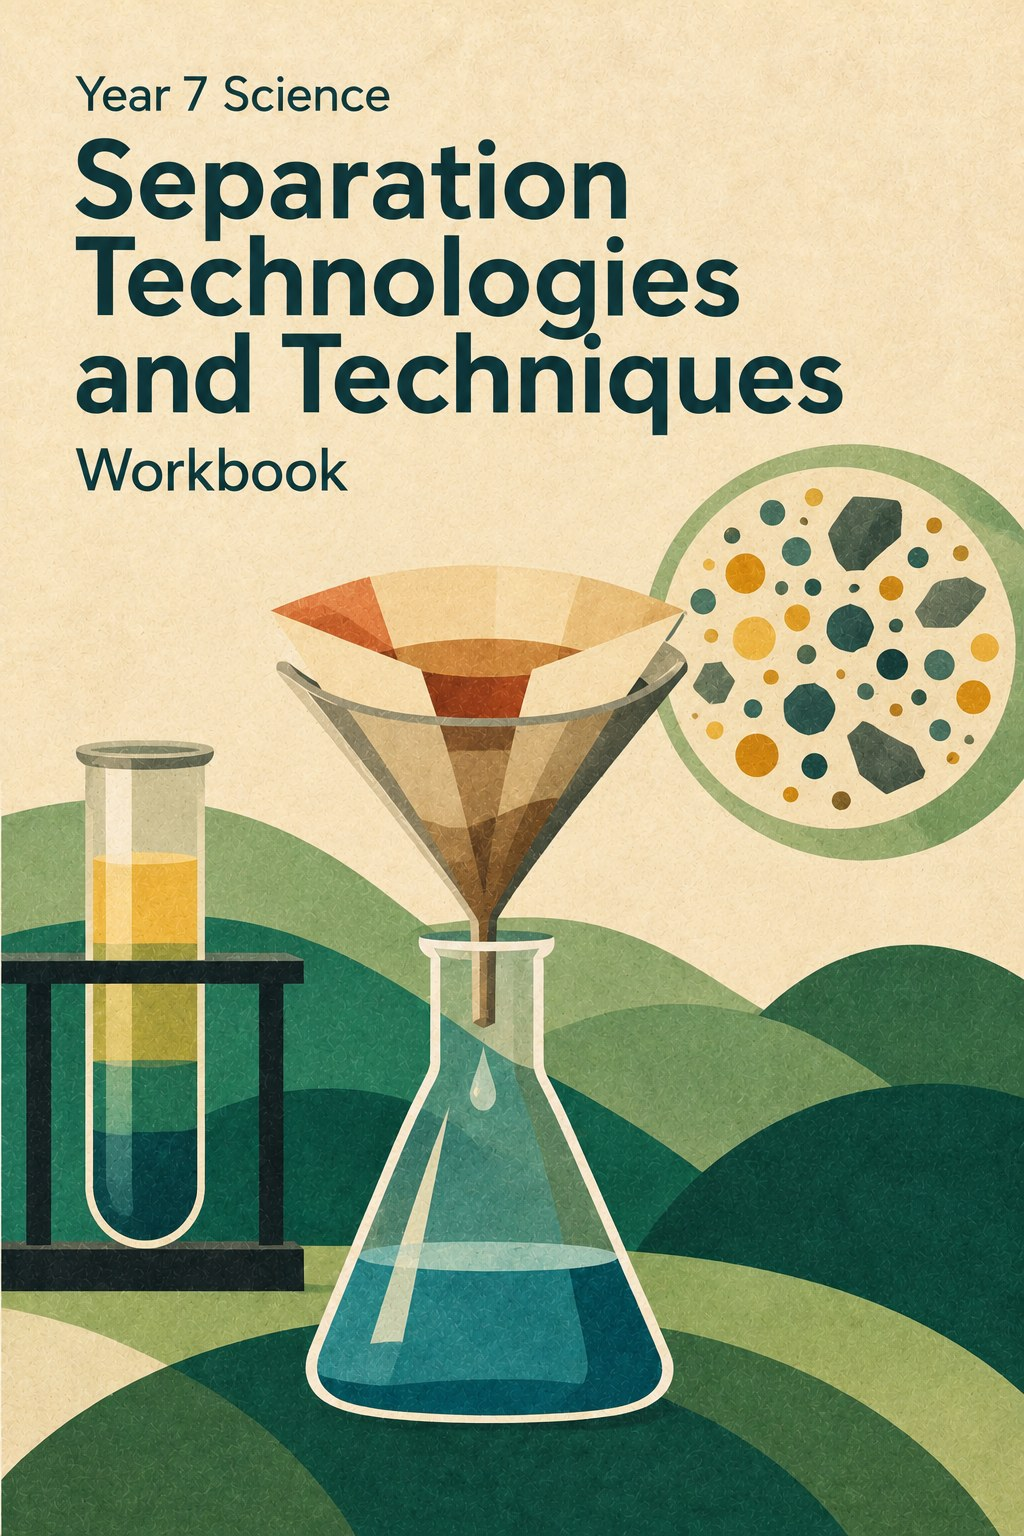
\includegraphics[width=\paperwidth]{../../../covers/separation.jpg}};
  \node[anchor=north east, fill=white, draw=Ink, line width=0.6pt, rounded corners=1.2mm,
        inner xsep=2mm, inner ysep=1.8mm, text width=30mm, font=\headingfont\footnotesize]
    at ([xshift=-4mm, yshift=-4mm]current page.north east)
    {\textbf{Name}\par\vspace{4mm}\hrule\vspace{2mm}\textbf{Class}\par\vspace{4mm}\hrule};
  \node[anchor=south east, fill=white, draw=Ink, line width=0.6pt, rounded corners=1.2mm,
        inner xsep=2.6mm, inner ysep=2mm, font=\headingfont\bfseries, align=right]
    at ([xshift=-4mm, yshift=6mm]current page.south east)
    {Advanced Separation\\[-1pt]{\normalfont\headingfont\scriptsize Topics 1--5}};
\end{tikzpicture}
\mbox{}
\clearpage

% ---- Inside cover ---------------------------------------------------------
\thispagestyle{plain}
{\headingfont\bfseries\fontsize{22}{26}\selectfont Advanced Separation}\par\vspace{1mm}
{\headingfont\large Topics 1--5 \textbullet\ Above the Year 7 level}\par\vspace{1mm}
{\small\itshape VC 2.0: VC2S8U06 \textbullet\ VC2S8U07 \textbullet\ VC2S10U07 \textbullet\ VC2S10H02--H03}\par\vspace{4mm}
\textbf{Teacher}\ \hrulefill\par

\begin{countrybox}{Acknowledgement of Country}
This booklet was created on the unceded Country of the Wurundjeri Woi-wurrung people of the Kulin Nation. We acknowledge Elders past, present and emerging.
\end{countrybox}

\begin{infobox}{How this booklet works}
\textbf{Advanced Separation} goes deeper into the ideas of the lesson books: more powerful models, the reasoning behind them, and harder problems that bring several ideas together. Each topic builds on the lessons named under its title. Each opens with its key vocabulary, then:\par\smallskip
\renewcommand{\arraystretch}{1.25}
\begin{tabular}{@{}p{24mm}p{70mm}@{}}
\textbf{Part A} & a reading with comprehension questions \\
\textbf{Part B} & the deeper idea, worked through \\
\textbf{Part C} & practice on your own \\
\textbf{Part D} & a challenge that pulls the ideas together \\
\end{tabular}

\smallskip
\begin{tabular}{@{}p{24mm}p{70mm}@{}}
\textbf{I do} \tagicon{\icodots{1}} & a worked example (solid frame) \\
\textbf{We do} \tagicon{\icodots{2}} & you try one with help (dashed frame) \\
\textbf{Reading} \tagicon{\icoread} & a passage to read (thin frame) \\
\end{tabular}
\end{infobox}

\clearpage
\markboth{Contents}{Contents}
{\headingfont\bfseries\LARGE Contents}\par\vspace{1mm}\noindent\rule{\linewidth}{0.6pt}\par\vspace{2mm}
\renewcommand{\arraystretch}{1.45}
\begin{tabular}{|C{1.1cm}|L{5.2cm}|C{1.7cm}|C{1.4cm}|}
  \hline\thead{Topic} & \thead{Title} & \thead{Deepens lesson} & \thead{Page} \\ \hline
  1 & \hyperlink{lesson.1.1}{Atoms, Elements and Compounds} & 1, 4 & \hyperlink{lesson.1.1}{p.\ \pageref{sec:1}} \\ \hline
  2 & \hyperlink{lesson.2.1}{Mixtures by Numbers} & 2, 5 & \hyperlink{lesson.2.1}{p.\ \pageref{sec:2}} \\ \hline
  3 & \hyperlink{lesson.3.1}{Separating by Size, Density and Magnetism} & 7 & \hyperlink{lesson.3.1}{p.\ \pageref{sec:3}} \\ \hline
  4 & \hyperlink{lesson.4.1}{Crystals and Solubility Curves} & 8, 10, 12 & \hyperlink{lesson.4.1}{p.\ \pageref{sec:4}} \\ \hline
  5 & \hyperlink{lesson.5.1}{Distillation and Chromatography at Work} & 16 & \hyperlink{lesson.5.1}{p.\ \pageref{sec:5}} \\ \hline
  --- & \hyperlink{glossary}{Glossary} & & \hyperlink{glossary}{\pageref{sec:glossary}} \\ \hline
\end{tabular}
\renewcommand{\arraystretch}{1}
\clearpage
\setcounter{section}{0}\renewcommand{\lessonart}{16}
\sectiondiv{Atoms, Elements and Compounds}{Dalton's atoms \textbullet{} The periodic table \textbullet{} Reading a formula \textbullet{} Why compounds are not mixtures}\label{sec:1}
\lessoncodes{Deepens Lessons 1 and 4 \textbullet{} VC2S8U07 \textbullet{} VC2S10U07}

\vocabhead
\begin{ctab}
\begin{tabular}{|SW{3.4cm}|W{7.0cm}|}
  \hline\hd & \thead{Word} & \thead{Definition (copy from the slide)} \\ \hline
  & \scaf{\textbf{Atom}\label{voc:atom}} & \scaf{The smallest particle of an element.} \\ \hline
  & \textbf{Periodic table}\label{voc:periodic-table} & \\ \hline
  & \textbf{Chemical symbol}\label{voc:chemical-symbol} & \\ \hline
  & \textbf{Chemical formula}\label{voc:chemical-formula} & \\ \hline
  & \textbf{Fixed ratio}\label{voc:fixed-ratio} & \\ \hline
\end{tabular}
\end{ctab}

\lessonpart{A}{Reading and comprehension}{Teal}\label{read:1}

\begin{readingbox}{Reading --- A Table With Gaps}
In 1808 the English teacher John Dalton argued that every element is made of its own kind of tiny, solid \textbf{atom}, and that compounds form when atoms of different elements join in simple whole-number ratios. Water, he said, is always the same combination, wherever it comes from. Experiments kept agreeing with him.

Scientists found more and more elements, and each was given a one- or two-letter \textbf{chemical symbol}: H for hydrogen, O for oxygen, Na for sodium (from its Latin name, \emph{natrium}). In 1869 the Russian chemist Dmitri Mendeleev arranged the 63 known elements in order of the mass of their atoms, in rows, so that elements with similar properties lined up in columns. Where the pattern did not fit, he left gaps, and predicted that new elements would be found to fill them. Within twenty years gallium and germanium were discovered, with almost exactly the properties he had predicted. His arrangement became the \textbf{periodic table}, which now holds 118 elements.

A \textbf{chemical formula} shows which atoms are joined in one particle of a compound, and how many of each. Because the atoms are always joined in the same \textbf{fixed ratio}, a compound always has the same make-up, unlike a mixture, which can be mixed in any proportion.
\end{readingbox}

\rcreset
\rcq{What were two of Dalton's ideas about atoms and compounds?}{2.5cm}
\rcq{Why did Mendeleev leave gaps in his table, and why was that a bold thing to do?}{3cm}
\rcq{Why is the symbol for sodium Na and not S?}{2cm}
\rcq{How is the make-up of a compound different from the make-up of a mixture?}{2.5cm}

\lessonpart{B}{Theory and examples}{Blue}\label{theory:1}

\subsection{Reading a Formula}\label{sub:a1.1}

\begin{skillbox}{Formulas}
Each capital letter starts a new element. A small number after a symbol counts the atoms of that element; no number means one. \quad H\textsubscript{2}O: 2 hydrogen, 1 oxygen.
\end{skillbox}

\begin{workedex}{Glucose, C\textsubscript{6}H\textsubscript{12}O\textsubscript{6}}
Carbon: 6 atoms. Hydrogen: 12. Oxygen: 6.\\
That is \textbf{3 elements} and $6 + 12 + 6 = \mathbf{24}$ atoms in each particle of glucose.
\end{workedex}

\begin{wedo}{Counting atoms}
For each compound, name the elements and count the atoms in one particle: ammonia, NH\textsubscript{3}; sulfuric acid, H\textsubscript{2}SO\textsubscript{4}; calcium carbonate (chalk), CaCO\textsubscript{3}.
\answerbox{5cm}
\end{wedo}

\subsection{A Compound Is Not a Mixture}\label{sub:a1.2}

\begin{workedex}{Table salt}
Sodium is a soft, shiny metal that fizzes violently in water. Chlorine is a poisonous green gas. Joined, they make sodium chloride, NaCl: table salt, which we eat every day.

\smallskip
A compound has \textbf{new properties}, unlike either element, and the atoms are joined in a fixed ratio (one sodium to one chlorine). In a mixture, each part keeps its own properties and can be in any proportion.
\end{workedex}

\begin{wedo}{Water}
Hydrogen is a gas that burns explosively. Oxygen is a gas that makes things burn more fiercely. Explain how water shows that it is a compound and not a mixture of these two gases. Give two pieces of evidence.
\answerbox{5cm}
\end{wedo}

\lessonpart{C}{Practice}{Amber}\label{prac:1}

\begin{keepext}
\needspace{10\baselineskip}
\task Scientists write a compound's \emph{formula} to show the atoms in each molecule. Water is H\textsubscript{2}O: two hydrogen atoms and one oxygen atom. Carbon dioxide is CO\textsubscript{2}.
\pt{a}How many atoms are in one molecule of carbon dioxide, and of which elements?
\answerbox{1.8cm}
\pt{b}Which of these diagrams could show carbon dioxide gas? Explain.
\begin{center}
\pboxfig{\pkinds{BB,BB,BB,BB,BB,BB,BB,BB}}{P}\hspace{6mm}%
\pboxfig{\pkinds{BAB,BAB,BAB,BAB,BAB,BAB,BAB,BAB}}{R}\hspace{6mm}%
\pboxfig{\pkinds{AA,BB,AA,BB,AA,BB,AA,BB}}{S}
\end{center}
\answerbox{2.0cm}
\end{keepext}

\begin{keepext}
\needspace{10\baselineskip}
\task Oxygen gas is made of molecules of two oxygen atoms, written O\textsubscript{2}. Is oxygen gas an element or a compound? Explain why it is still a pure substance.
\answerbox{2.8cm}
\end{keepext}

\begin{keepext}
\needspace{10\baselineskip}
\task Gold jewellery is often 18-carat, which means it is 75\% gold mixed with other metals. Suggest one reason jewellers mix gold with other metals, and explain whether 18-carat gold is a pure substance.
\answerbox{3.0cm}
\end{keepext}

\begin{keepext}
\needspace{10\baselineskip}
\task Draw a particle diagram of a pure compound whose molecules each contain one red atom joined to two blue atoms. Use red and blue circles, or label them R and B.
\drawbox{5cm}{}
\end{keepext}


\begin{keepext}
\needspace{10\baselineskip}
\task Add a third question to the flowchart for pure substances: ``Is each particle made of one kind of atom, or more than one kind?'' Write the two answers it leads to.
\answerbox{2.4cm}
\end{keepext}

\begin{keepext}
\needspace{12\baselineskip}
\task Classify each diagram as an element, a compound, or a mixture.
\begin{center}
\pboxfig{\pkinds{BB,BB,BB,BB,BB,BB,BB,BB}}{X}\hspace{6mm}%
\pboxfig{\pkinds{BAB,BAB,BAB,BAB,BAB,BAB,BAB,BAB}}{Y}\hspace{6mm}%
\pboxfig{\pkinds{BB,BAB,BB,BAB,BB,BAB,BB,BAB}}{Z}
\end{center}
\begin{ctab}
\begin{tabular}{|SZ{3.51cm}|Z{3.51cm}|Z{3.51cm}|}
  \hd & \thead{X} & \thead{Y} & \thead{Z} \\ \hline
  & & & \\ \hline
\end{tabular}
\end{ctab}
\end{keepext}

\begin{keepext}
\needspace{10\baselineskip}
\task Air contains nitrogen (N\textsubscript{2}), oxygen (O\textsubscript{2}) and carbon dioxide (CO\textsubscript{2}). Draw a particle diagram of air with a key. Show the right kinds of molecule, and more nitrogen than anything else.
\drawbox{5cm}{}
\end{keepext}


\lessonpart{D}{Challenge}{Violet}\label{ext:1}

\task Every 18\,g of pure water, from anywhere, contains 2\,g of hydrogen and 16\,g of oxygen.
\pt{a} How much hydrogen and how much oxygen are in 45\,g of water? Show your working.
\workbox{4cm}
\pt{b} A container of hydrogen and oxygen \emph{gases} can hold the two in any ratio. Explain why water cannot, using the idea of atoms joined in a fixed ratio.
\answerbox{4.5cm}

\clearpage

% ══════════════════════════════════════════════════════════════════════════════
%  TOPIC 2 — MIXTURES BY NUMBERS                         (deepens Lessons 2, 5)
% ══════════════════════════════════════════════════════════════════════════════
\setcounter{section}{1}\renewcommand{\lessonart}{19}
\sectiondiv{Mixtures by Numbers}{Concentration in g/L \textbullet{} Dilution \textbullet{} Very small amounts: parts per million}\label{sec:2}
\lessoncodes{Deepens Lessons 2 and 5 \textbullet{} VC2S8U06 \textbullet{} VC2S10I04}

\vocabhead
\begin{ctab}
\begin{tabular}{|SW{3.4cm}|W{7.0cm}|}
  \hline\hd & \thead{Word} & \thead{Definition (copy from the slide)} \\ \hline
  & \scaf{\textbf{Concentration}\label{voc:concentration}} & \scaf{How much solute is dissolved in a given volume of solution.} \\ \hline
  & \textbf{Grams per litre (g/L)}\label{voc:grams-per-litre-g-l} & \\ \hline
  & \textbf{Dilute (verb)}\label{voc:dilute-verb} & \\ \hline
  & \textbf{Percentage by mass}\label{voc:percentage-by-mass} & \\ \hline
  & \textbf{Parts per million (ppm)}\label{voc:parts-per-million-ppm} & \\ \hline
\end{tabular}
\end{ctab}

\lessonpart{A}{Reading and comprehension}{Teal}\label{read:2}

\begin{readingbox}{Reading --- How Much Is in There?}
``Strong'' and ``weak'' are fine words in the kitchen, but a chemist, a nurse or a water engineer needs numbers. The \textbf{concentration} of a solution says how much solute is in a set volume of it. One common unit is \textbf{grams per litre} (g/L): the mass of solute in every litre of solution. Sea water is about 35\,g/L of salt.

To \textbf{dilute} a solution, you add more solvent. The amount of solute does not change, but it is spread through a bigger volume, so the concentration falls. Cordial, cleaning products and medicines are all diluted before use, and the instructions are written so the right concentration is reached.

Mixtures of solids are often described by \textbf{percentage by mass}: 18-carat gold is 75\% gold by mass. For very small amounts, scientists use \textbf{parts per million} (ppm). One ppm is one gram of something in a million grams of mixture, or about one milligram in a litre of water. Melbourne's tap water has fluoride added at about 1\,ppm to protect teeth; drinking-water rules limit lead to less than 0.01\,ppm.
\end{readingbox}

\rcreset
\rcq{Why do scientists describe concentration with numbers instead of ``strong'' or ``weak''?}{2.5cm}
\rcq{What stays the same, and what changes, when a solution is diluted?}{2.5cm}
\rcq{What does 1\,ppm mean?}{2cm}
\rcq{Why is ppm a better unit than g/L for the lead in drinking water?}{2.5cm}

\lessonpart{B}{Theory and examples}{Blue}\label{theory:2}

\subsection{Concentration in g/L}\label{sub:a2.1}

\begin{skillbox}{Concentration}
\[ \text{concentration (g/L)} = \frac{\text{mass of solute (g)}}{\text{volume of solution (L)}} \qquad 1\,\text{L} = 1000\,\text{mL} \]
\end{skillbox}

\begin{workedex}{Sugar in water}
25\,g of sugar is dissolved to make 500\,mL of solution.

\smallskip
$500\,\text{mL} = 0.5\,\text{L}$. \quad Concentration $= 25 \div 0.5 = \mathbf{50\ g/L}$.
\end{workedex}

\begin{wedo}{A sports drink}
A 600\,mL bottle of sports drink contains 36\,g of sugar. Find its concentration in g/L. Is it more or less concentrated than the worked example?
\workbox{4cm}
\end{wedo}

\subsection{Dilution}\label{sub:a2.2}

\begin{workedex}{Making up cordial}
200\,mL of cordial with a sugar concentration of 100\,g/L is topped up with water to 1\,L. Find the new concentration.

\smallskip
Sugar in the cordial: $100 \times 0.2 = 20$\,g. Diluting does not change this.\\
New concentration $= 20 \div 1 = \mathbf{20\ g/L}$: five times the volume, one-fifth the concentration.
\end{workedex}

\begin{wedo}{Diluting salt water}
50\,mL of salt water at 40\,g/L is diluted to 250\,mL. Find the mass of salt and the new concentration.
\workbox{4.5cm}
\end{wedo}

\lessonpart{C}{Practice}{Amber}\label{prac:2}

\begin{keepext}
\needspace{10\baselineskip}
\task Air is about 78\% nitrogen, 21\% oxygen and 1\% other gases.
\pt{a}In a particle diagram of 100 air particles, how many should be oxygen?
\answerbox{1.4cm}
\pt{b}Is a diagram with half nitrogen and half oxygen a good model of air? Explain.
\answerbox{2.0cm}
\end{keepext}

\begin{keepext}
\needspace{10\baselineskip}
\task Milk looks uniform, but under a strong microscope you can see tiny droplets of fat spread through the water. Should milk be called uniform or non-uniform? Explain why the answer depends on how closely you look.
\answerbox{3.0cm}
\end{keepext}

\begin{keepext}
\needspace{10\baselineskip}
\task Stainless steel is a uniform mixture of iron, chromium and a little nickel. It does not rust, but pure iron does. Does this mean the components have lost their properties? Suggest what is happening.
\answerbox{3.0cm}
\end{keepext}

\begin{keepext}
\needspace{10\baselineskip}
\task A recipe needs 250\,g of a mixture that is 20\% sugar. How many grams of sugar and how many grams of other ingredients are needed? Show your working.
\workbox{2.6cm}
\end{keepext}


\begin{keepext}
\needspace{10\baselineskip}
\task Concentration can be written as grams of solute per 100\,mL of solution. Solution A has 30\,g of sugar in 200\,mL. Solution B has 20\,g in 100\,mL. Calculate the concentration of each, in g per 100\,mL, and say which is more concentrated.
\workbox{3.0cm}
\end{keepext}

\begin{keepext}
\needspace{10\baselineskip}
\task 50\,mL of water and 50\,mL of ethanol are mixed. The total volume is only about 96\,mL, but the total mass does not change. Use the particle model to suggest why the volume shrinks.
\answerbox{3.0cm}
\end{keepext}

\begin{keepext}
\needspace{10\baselineskip}
\task Gases can dissolve in liquids too. Name the gas dissolved in a fizzy drink, and explain why bubbles appear when the bottle is opened.
\answerbox{2.8cm}
\end{keepext}

\begin{keepext}
\needspace{10\baselineskip}
\task Fish breathe oxygen that is dissolved in water. In summer, when water is warm, fish in shallow ponds sometimes struggle. Suggest why, given that less oxygen can dissolve in warm water than in cold.
\answerbox{2.8cm}
\end{keepext}


\lessonpart{D}{Challenge}{Violet}\label{ext:2}

\task Melbourne's tap water contains about 1\,ppm of fluoride, that is, about 1\,mg in each litre.
\pt{a} A student drinks 2\,L of tap water a day. How many milligrams of fluoride is that in a year? Give your answer in grams too. (1\,g $=$ 1000\,mg.)
\workbox{4cm}
\pt{b} A dentist says the amount is safe and helps teeth, but much more would harm them. Explain why it matters that the water authority measures and controls the concentration, not just whether fluoride is present.
\answerbox{4.5cm}

\clearpage

% ══════════════════════════════════════════════════════════════════════════════
%  TOPIC 3 — SEPARATING BY SIZE, DENSITY AND MAGNETISM       (deepens Lesson 7)
% ══════════════════════════════════════════════════════════════════════════════
\setcounter{section}{2}\renewcommand{\lessonart}{25}
\sectiondiv{Separating by Size, Density and Magnetism}{Choosing a method from a property \textbullet{} Separating in several steps \textbullet{} Sedimentation and the centrifuge}\label{sec:3}
\lessoncodes{Deepens Lesson 7 \textbullet{} VC2S8U06 \textbullet{} VC2S10H02}

\vocabhead
\begin{ctab}
\begin{tabular}{|SW{3.4cm}|W{7.0cm}|}
  \hline\hd & \thead{Word} & \thead{Definition (copy from the slide)} \\ \hline
  & \scaf{\textbf{Sedimentation}\label{voc:sedimentation}} & \scaf{Letting heavier, denser solid particles settle to the bottom of a liquid.} \\ \hline
  & \textbf{Sediment}\label{voc:sediment} & \\ \hline
  & \textbf{Centrifuge}\label{voc:centrifuge} & \\ \hline
  & \textbf{Sieve}\label{voc:sieve} & \\ \hline
  & \textbf{Flocculant}\label{voc:flocculant} & \\ \hline
\end{tabular}
\end{ctab}

\lessonpart{A}{Reading and comprehension}{Teal}\label{read:3}

\begin{readingbox}{Reading --- From River to Tap}
Water from a reservoir carries fine clay and silt that would take weeks to settle. At a water treatment plant, a \textbf{flocculant} is stirred in. It makes the tiny particles clump into larger, heavier flakes. In big settling tanks the flakes sink: this is \textbf{sedimentation}, and the layer that forms on the bottom is the \textbf{sediment}. The clearer water above flows over the top, then through filters of sand and gravel.

When a mixture will not settle quickly enough, scientists spin it. A \textbf{centrifuge} whirls test tubes around hundreds of times a second. The spinning acts like extra-strong gravity, so the denser parts are flung to the bottom in minutes. A blood sample spun in a centrifuge separates into a layer of red cells at the bottom and pale yellow plasma on top. Dairies use the same idea to separate cream from milk.

Many real mixtures need several steps. A \textbf{sieve} sorts by particle size, a magnet removes iron and steel, water dissolves what is soluble, and density lets light and heavy parts be washed or spun apart. Engineers choose the order so each step leaves an easier mixture for the next.
\end{readingbox}

\rcreset
\rcq{What does a flocculant do, and why does it make sedimentation faster?}{2.5cm}
\rcq{Why does spinning in a centrifuge separate a mixture faster than leaving it to settle?}{2.5cm}
\rcq{Describe what a blood sample looks like after it has been spun.}{2cm}
\rcq{Why must engineers think about the order of the steps?}{2.5cm}

\lessonpart{B}{Theory and examples}{Blue}\label{theory:3}

\subsection{Choosing a Method from a Property}\label{sub:a3.1}

\begin{ctab}
\begin{tabular}{|W{3.6cm}|W{6.6cm}|}
  \hline\thead{Property that differs} & \thead{Methods that use it} \\ \hline
  Particle size & sieving, filtering \\ \hline
  Density & decanting, sedimentation, centrifuging, panning \\ \hline
  Magnetism & magnetic separation \\ \hline
  Solubility & dissolving, then filtering \\ \hline
  Boiling point & evaporation, distillation \\ \hline
\end{tabular}
\end{ctab}

\begin{workedex}{Sand, iron filings and salt}
\textbf{1.} Draw a magnet through the dry mixture: the iron filings stick to it (magnetism). \textbf{2.} Stir the rest into water: the salt dissolves, the sand does not (solubility). \textbf{3.} Filter: the sand is the residue (particle size). \textbf{4.} Evaporate the filtrate: salt is left (boiling point).
\end{workedex}

\begin{wedo}{Four ingredients}
A mixture contains rice grains, sand, salt and iron filings. Plan the steps to separate all four, in order. For each step, name the property it uses.
\answerbox{6cm}
\end{wedo}

\subsection{Sedimentation and the Centrifuge}\label{sub:a3.2}

\begin{workedex}{Muddy water}
Muddy water is left in a jar. After an hour the sand has settled but the water is still cloudy. Explain.

\smallskip
Sand grains are large and dense, so they sink quickly. The clay particles are so tiny that the water's moving particles keep bumping them around, and they sink extremely slowly. A flocculant, a filter or a centrifuge would be needed to clear the water.
\end{workedex}

\begin{wedo}{Spinning blood}
After a blood sample is spun, the red cells are at the bottom and the plasma at the top. Which part is denser? Explain why a hospital spins blood instead of leaving it to settle.
\answerbox{4.5cm}
\end{wedo}

\lessonpart{C}{Practice}{Amber}\label{prac:3}

\begin{keepext}
\needspace{10\baselineskip}
\task Gold panning is a way to find gold in river gravel. The miner swirls gravel and water in a shallow pan and washes the lighter material over the edge. Gold has a density of 19.3\,g/cm\textsuperscript{3}; most sand and gravel is about 2.6\,g/cm\textsuperscript{3}. Explain why the gold is left behind, and name the separation technique it is most like.
\answerbox{3.2cm}
\end{keepext}

\begin{keepext}
\needspace{10\baselineskip}
\task A recycling plant has a mixture of steel cans, aluminium cans and plastic bottles. A magnet removes only the steel. Suggest a property that could be used to separate the aluminium from the plastic, and explain how.
\answerbox{3.0cm}
\end{keepext}

\begin{keepext}
\needspace{10\baselineskip}
\task A student filters 50\,g of a sand and salt mixture after stirring it into water. The dried residue has a mass of 32\,g. What mass of salt was in the mixture? What percentage of the mixture was salt?
\workbox{3.0cm}
\end{keepext}

\begin{keepext}
\needspace{10\baselineskip}
\task Our kidneys filter the blood. Blood cells are too big to pass through the filter, but water, salts and waste can. Compare this with filtering sand from salt water: what plays the part of the residue, and what the filtrate?
\answerbox{3.0cm}
\end{keepext}


\lessonpart{D}{Challenge}{Violet}\label{ext:3}

\task A recycling plant receives a crushed mixture of steel, aluminium, glass and paper. Design a flow chart of steps to separate all four. For each step, name the method and the property it uses, and explain why your order works.
\answerbox{9cm}

\clearpage

% ══════════════════════════════════════════════════════════════════════════════
%  TOPIC 4 — CRYSTALS AND SOLUBILITY CURVES          (deepens Lessons 8, 10, 12)
% ══════════════════════════════════════════════════════════════════════════════
\setcounter{section}{3}\renewcommand{\lessonart}{21}
\sectiondiv{Crystals and Solubility Curves}{Reading a solubility curve \textbullet{} How much crystallises? \textbullet{} Big crystals, small crystals \textbullet{} Purifying by recrystallisation}\label{sec:4}
\lessoncodes{Deepens Lessons 8, 10 and 12 \textbullet{} VC2S8U06 \textbullet{} VC2S10I05}

\vocabhead
\begin{ctab}
\begin{tabular}{|SW{3.4cm}|W{7.0cm}|}
  \hline\hd & \thead{Word} & \thead{Definition (copy from the slide)} \\ \hline
  & \scaf{\textbf{Solubility curve}\label{voc:solubility-curve}} & \scaf{A graph of how much solute dissolves in 100\,g of water at each temperature.} \\ \hline
  & \textbf{Crystal lattice}\label{voc:crystal-lattice} & \\ \hline
  & \textbf{Recrystallisation}\label{voc:recrystallisation} & \\ \hline
  & \textbf{Impurity}\label{voc:impurity} & \\ \hline
  & \textbf{Rate of cooling}\label{voc:rate-of-cooling} & \\ \hline
\end{tabular}
\end{ctab}

\lessonpart{A}{Reading and comprehension}{Teal}\label{read:4}

\begin{readingbox}{Reading --- Slow Cooling, Big Crystals}
Look closely at salt or sugar and you will see tiny cubes and blocks with flat faces. Their shape comes from the way the particles stack in a regular, repeating pattern called a \textbf{crystal lattice}. As a solution cools or evaporates, particles join the lattice one layer at a time.

How big the crystals grow depends on the \textbf{rate of cooling}. Cool a solution slowly and particles have time to find their places on a few growing crystals, so they become large. Cool it fast and many tiny crystals start at once. The same is true of rocks: granite cooled slowly deep underground and has crystals you can see; basalt cooled quickly at the surface and its crystals are tiny.

Factories use crystals to make substances purer. Raw sugar is dissolved in hot water, filtered, and cooled. The sugar crystallises out, while most of the \textbf{impurities}, being only a small amount, stay dissolved. This is \textbf{recrystallisation}. A \textbf{solubility curve} tells chemists exactly how much will crystallise at each temperature.
\end{readingbox}

\rcreset
\rcq{What gives a crystal its flat faces and regular shape?}{2.5cm}
\rcq{Why does slow cooling make larger crystals?}{2.5cm}
\rcq{Explain why granite and basalt have different crystal sizes.}{2.5cm}
\rcq{Why do the impurities stay in solution during recrystallisation?}{2.5cm}

\lessonpart{B}{Theory and examples}{Blue}\label{theory:4}

\subsection{How Much Crystallises?}\label{sub:a4.1}

\begin{center}
\begin{fitbox}\begin{tikzpicture}[font=\small, x=0.11cm, y=0.024cm]
  \draw[->, line width=0.7pt] (0,0) -- (88,0) node[pos=0.5, below=11pt, font=\scriptsize] {temperature (\textdegree C)};
  \draw[->, line width=0.7pt] (0,0) -- (0,185) node[above right, font=\scriptsize] {g per 100\,g of water};
  \foreach \x in {0,20,40,60,80} \draw (\x,0) -- (\x,-4) node[below, font=\scriptsize] {\x};
  \foreach \y in {0,40,80,120,160} \draw (0,\y) -- (-1.2,\y) node[left, font=\scriptsize] {\y};
  \foreach \y in {40,80,120,160} \draw[black!15] (0,\y) -- (85,\y);
  \draw[line width=1.2pt] plot[smooth] coordinates {(0,13) (20,32) (40,64) (60,110) (80,169)};
  \node[font=\scriptsize, anchor=east] at (56,140) {potassium nitrate};
  \draw[line width=1.2pt, densely dashed] (0,36) -- (80,38);
  \node[font=\scriptsize, anchor=west] at (55,25) {salt};
\end{tikzpicture}\end{fitbox}
\figcap{Solubility of potassium nitrate (solid) and salt (dashed).}
\end{center}

\begin{workedex}{Cooling a saturated solution}
100\,g of water is saturated with potassium nitrate at 60\,\textdegree C and cooled to 20\,\textdegree C. What mass of crystals forms?

\smallskip
At 60\,\textdegree C it holds 110\,g; at 20\,\textdegree C only 32\,g. The rest comes out as crystals: $110 - 32 = \mathbf{78\ g}$.
\end{workedex}

\begin{wedo}{Half the water}
50\,g of water is saturated with potassium nitrate at 40\,\textdegree C and cooled to 20\,\textdegree C. Use the graph to find the mass of crystals. (Hint: 50\,g of water holds half as much as 100\,g.)
\workbox{5cm}
\end{wedo}

\subsection{Big Crystals, Small Crystals}\label{sub:a4.2}

\begin{workedex}{Rock candy}
Sugar syrup left on a windowsill for a week grows large crystals on a string. The same syrup put in a freezer forms a grainy paste of tiny crystals. Explain.

\smallskip
On the windowsill water evaporates slowly, so sugar particles join a few crystals one by one and they grow large. In the freezer the syrup cools quickly, so crystals start in thousands of places at once and none can grow big.
\end{workedex}

\begin{wedo}{Two igneous rocks}
Rock X has crystals several millimetres across; rock Y looks smooth, with crystals too small to see. Both formed from the same molten rock. Which cooled underground and which in a lava flow? Explain.
\answerbox{4.5cm}
\end{wedo}

\lessonpart{C}{Practice}{Amber}\label{prac:4}

\begin{keepext}
\needspace{10\baselineskip}
\task When a copper sulfate solution is evaporated to dryness with strong heat, the blue solid left behind turns into a white powder. Suggest why crystallisation is a better method for this substance.
\answerbox{3.0cm}
\end{keepext}

\begin{keepext}
\needspace{10\baselineskip}
\task Sea water is about 3.5\% salt by mass. What mass of salt is in 2\,kg (2000\,g) of sea water? How much sea water would a salt pan need to evaporate to produce 1\,kg of salt?
\workbox{3.2cm}
\end{keepext}

\begin{keepext}
\needspace{10\baselineskip}
\task Plan how to grow the largest possible crystal of salt at home. Describe what you would do, and explain how each step helps the crystal grow large.
\answerbox{3.4cm}
\end{keepext}

\begin{keepext}
\needspace{10\baselineskip}
\task Leaching cycad seeds took days and needed a lot of water. Suggest two things that would make leaching faster, and explain each using the particle model of dissolving.
\answerbox{3.0cm}
\end{keepext}


\begin{keepext}
\needspace{10\baselineskip}
\task You need to make exactly 300\,g of saturated salt solution at 20\,\textdegree C (solubility 36\,g per 100\,g of water). How much water and how much salt do you need? Hint: start with the mass of solution made from 100\,g of water.
\workbox{3.2cm}
\end{keepext}

\begin{keepext}
\needspace{10\baselineskip}
\task Gases are the opposite of most solids: they are \emph{less} soluble in warm water. Use the particle model to suggest why a gas escapes from warm water more easily.
\answerbox{3.0cm}
\end{keepext}

\begin{keepext}
\needspace{10\baselineskip}
\task A ``supersaturated'' solution holds more solute than it should at its temperature. If a single small crystal is dropped in, crystals suddenly spread through the whole solution. Suggest why.
\answerbox{3.0cm}
\end{keepext}

\begin{keepext}
\needspace{10\baselineskip}
\task Plan a fair test to compare how soluble salt and sugar are at room temperature. Describe what you would measure, and two things you would keep the same.
\answerbox{3.2cm}
\end{keepext}


\begin{keepext}
\needspace{10\baselineskip}
\task A saturated solution of potassium nitrate is made in 50\,g of water at 80\,\textdegree C (solubility 169\,g per 100\,g of water) and cooled to 20\,\textdegree C (32\,g per 100\,g). What mass of crystals forms? Show your working.
\workbox{3.2cm}
\end{keepext}

\begin{keepext}
\needspace{10\baselineskip}
\task Cooling a salt solution from 80\,\textdegree C to 20\,\textdegree C produces only about 2\,g of crystals per 100\,g of water (38\,g down to 36\,g). Suggest a better way to get salt crystals out of salt water, and explain why it works better.
\answerbox{3.0cm}
\end{keepext}

\begin{keepext}
\needspace{10\baselineskip}
\task A mixture contains 60\,g of potassium nitrate and 10\,g of salt, dissolved in 100\,g of water at 80\,\textdegree C. It is cooled to 20\,\textdegree C. At 20\,\textdegree C, 32\,g of potassium nitrate and 36\,g of salt can stay dissolved in 100\,g of water. Which substance crystallises out, and how much? Explain how this could be used to purify potassium nitrate.
\answerbox{3.4cm}
\end{keepext}


\lessonpart{D}{Challenge}{Violet}\label{ext:4}

\task A sample of potassium nitrate is contaminated with sand and a small amount of salt. Using the solubility curve, plan a method to get pure, dry potassium nitrate crystals. Give the temperatures you would use, explain how each step removes one of the impurities, and say why a little potassium nitrate will always be lost.
\answerbox{9cm}

\clearpage

% ══════════════════════════════════════════════════════════════════════════════
%  TOPIC 5 — DISTILLATION AND CHROMATOGRAPHY AT WORK        (deepens Lesson 16)
% ══════════════════════════════════════════════════════════════════════════════
\setcounter{section}{4}\renewcommand{\lessonart}{27}
\sectiondiv{Distillation and Chromatography at Work}{Fractional distillation \textbullet{} Oil refineries and liquid air \textbullet{} $R_f$ values in forensic science \textbullet{} Making fresh water}\label{sec:5}
\lessoncodes{Deepens Lesson 16 \textbullet{} VC2S8U06 \textbullet{} VC2S10H02 \textbullet{} VC2S10H03}

\vocabhead
\begin{ctab}
\begin{tabular}{|SW{3.4cm}|W{7.0cm}|}
  \hline\hd & \thead{Word} & \thead{Definition (copy from the slide)} \\ \hline
  & \scaf{\textbf{Fractional distillation}\label{voc:fractional-distillation}} & \scaf{Separating a mixture of liquids with different boiling points, using a tall column, into parts called fractions.} \\ \hline
  & \textbf{Fraction}\label{voc:fraction} & \\ \hline
  & \textbf{Crude oil}\label{voc:crude-oil} & \\ \hline
  & \textbf{$R_f$ value}\label{voc:r-f-value} & \\ \hline
  & \textbf{Reverse osmosis}\label{voc:reverse-osmosis} & \\ \hline
\end{tabular}
\end{ctab}

\lessonpart{A}{Reading and comprehension}{Teal}\label{read:5}

\begin{readingbox}{Reading --- Separating on a Giant Scale}
\textbf{Crude oil} pumped from the ground is a thick, dark mixture of hundreds of substances. At a refinery it is heated until most of it boils, and the vapour rises up a tower many storeys tall that is hot at the bottom and cooler at the top. Each substance condenses back into a liquid at the height where the tower is cool enough for it. Trays at different heights collect each \textbf{fraction}: gases for cooking at the top, then petrol, kerosene for jet fuel, diesel, and thick bitumen for roads at the bottom. This is \textbf{fractional distillation}.

The air you breathe is separated the same way, but the other way round: air is cooled to about $-200$\,\textdegree C until it becomes a liquid, and then allowed to warm. Nitrogen boils off first, at $-196$\,\textdegree C, then oxygen at $-183$\,\textdegree C. Hospitals use the oxygen.

Chromatography works on tiny samples. Forensic scientists use it to match an ink to a pen, and sports drug testers use it to find banned substances in a drop of urine. Each substance travels a set fraction of the distance the solvent travels, its \textbf{$R_f$ value}, so it can be identified like a fingerprint.

Victoria's desalination plant at Wonthaggi does not distil sea water. It uses \textbf{reverse osmosis}: sea water is pushed at high pressure through a membrane whose pores let water particles through but hold the salt back.
\end{readingbox}

\rcreset
\rcq{Why does each fraction collect at a different height in the tower?}{2.5cm}
\rcq{In which order do nitrogen and oxygen boil off as liquid air warms? Why?}{2.5cm}
\rcq{Give two uses of chromatography outside a school lab.}{2cm}
\rcq{How does reverse osmosis separate salt from water?}{2.5cm}

\lessonpart{B}{Theory and examples}{Blue}\label{theory:5}

\subsection{Fractional Distillation}\label{sub:a5.1}

\begin{workedex}{Three liquids}
A mixture contains pentane (boils at 36\,\textdegree C), hexane (69\,\textdegree C) and heptane (98\,\textdegree C). It is heated slowly in a fractionating column. In what order are they collected?

\smallskip
The lowest boiling point boils first and reaches the top of the column: \textbf{pentane}, then \textbf{hexane}, then \textbf{heptane}. The thermometer stays near 36\,\textdegree C while pentane distils, then rises towards 69\,\textdegree C.
\end{workedex}

\begin{wedo}{Liquid air}
Liquid air contains nitrogen (boils at $-196$\,\textdegree C), argon ($-186$\,\textdegree C) and oxygen ($-183$\,\textdegree C). In what order do they boil off as it warms? Explain why argon and oxygen are the hardest pair to separate.
\answerbox{4.5cm}
\end{wedo}

\subsection{$R_f$ Values}\label{sub:a5.2}

\begin{skillbox}{$R_f$ value}
\[ R_f = \frac{\text{distance moved by the spot}}{\text{distance moved by the solvent front}} \]
Both distances are measured from the starting line. The same substance, with the same paper and solvent, always has the same $R_f$.
\end{skillbox}

\begin{workedex}{Matching a dye}
A spot moved 2.4\,cm while the solvent front moved 6.0\,cm. $R_f = 2.4 \div 6.0 = \mathbf{0.40}$. Known dyes: yellow 0.25, red 0.40, blue 0.70. The spot is the \textbf{red} dye.
\end{workedex}

\begin{wedo}{A forged signature}
Ink from a forged cheque gave two spots, 1.5\,cm and 4.8\,cm from the start, with the solvent front at 6.0\,cm. Pen P's ink has spots with $R_f$ 0.25 and 0.80; pen Q's has 0.25 and 0.60. Which pen was used? Show your working.
\workbox{5cm}
\end{wedo}

\lessonpart{C}{Practice}{Amber}\label{prac:5}

\begin{keepext}
\needspace{10\baselineskip}
\task Scientists compare spots using the $R_f$ value: the distance the spot moved divided by the distance the solvent front moved. A dye moved 3.0\,cm while the solvent front moved 7.5\,cm. Calculate its $R_f$ value. Why must every $R_f$ value be less than 1?
\workbox{2.6cm}
\end{keepext}

\begin{keepext}
\needspace{10\baselineskip}
\task Ethanol boils at 78\,\textdegree C and water at 100\,\textdegree C. A mixture of the two is heated slowly, and the thermometer at the top of the flask is watched. Describe what you would expect the thermometer to show, and explain how this lets you collect mostly ethanol first.
\answerbox{3.4cm}
\end{keepext}

\begin{keepext}
\needspace{10\baselineskip}
\task Distillation needs a lot of energy because water must be boiled. Suggest one way a solar still in the desert could make drinking water without fuel. Sketch and label your idea.
\drawbox{5.5cm}{}
\end{keepext}


\lessonpart{D}{Challenge}{Violet}\label{ext:5}

\task A remote island has plenty of sunshine and sea water, but no electricity grid and little fuel. Compare distillation and reverse osmosis as ways to make its drinking water: what each needs, and its advantages and disadvantages. Recommend one, and justify your choice.
\answerbox{9cm}

\clearpage

\clearpage\markboth{Glossary}{Glossary}\hypertarget{glossary}{}\pdfbookmark[1]{Glossary}{glossarybm}
{\headingfont\bfseries\LARGE Glossary}\label{sec:glossary}\par\vspace{1mm}\noindent\rule{\linewidth}{0.6pt}\par
{\small Every key word in this booklet and the page it is introduced on.}\par\smallskip
\renewcommand{\arraystretch}{1.3}
\begin{longtable}{|>{\RaggedRight}p{34mm}|p{9mm}|p{\dimexpr\linewidth-43mm-6\tabcolsep-4\arrayrulewidth-1pt\relax}|}
\hline \rule{0pt}{4mm}\headingfont\bfseries Word & \headingfont\bfseries Page & \headingfont\bfseries In my own words \\ \hline \endhead
  $R_f$ value & \pageref{voc:r-f-value} & \\ \hline
  Atom & \pageref{voc:atom} & \\ \hline
  Centrifuge & \pageref{voc:centrifuge} & \\ \hline
  Chemical formula & \pageref{voc:chemical-formula} & \\ \hline
  Chemical symbol & \pageref{voc:chemical-symbol} & \\ \hline
  Concentration & \pageref{voc:concentration} & \\ \hline
  Crude oil & \pageref{voc:crude-oil} & \\ \hline
  Crystal lattice & \pageref{voc:crystal-lattice} & \\ \hline
  Dilute (verb) & \pageref{voc:dilute-verb} & \\ \hline
  Fixed ratio & \pageref{voc:fixed-ratio} & \\ \hline
  Flocculant & \pageref{voc:flocculant} & \\ \hline
  Fraction & \pageref{voc:fraction} & \\ \hline
  Fractional distillation & \pageref{voc:fractional-distillation} & \\ \hline
  Grams per litre (g/L) & \pageref{voc:grams-per-litre-g-l} & \\ \hline
  Impurity & \pageref{voc:impurity} & \\ \hline
  Parts per million (ppm) & \pageref{voc:parts-per-million-ppm} & \\ \hline
  Percentage by mass & \pageref{voc:percentage-by-mass} & \\ \hline
  Periodic table & \pageref{voc:periodic-table} & \\ \hline
  Rate of cooling & \pageref{voc:rate-of-cooling} & \\ \hline
  Recrystallisation & \pageref{voc:recrystallisation} & \\ \hline
  Reverse osmosis & \pageref{voc:reverse-osmosis} & \\ \hline
  Sediment & \pageref{voc:sediment} & \\ \hline
  Sedimentation & \pageref{voc:sedimentation} & \\ \hline
  Sieve & \pageref{voc:sieve} & \\ \hline
  Solubility curve & \pageref{voc:solubility-curve} & \\ \hline
\end{longtable}
\padtofour
\end{document}
